%%%%%%%%%%%%%%%%%%%%%%%%%%%%%%%%%%%%%%%%%
% The Legrand Orange Book
% LaTeX Template
% Version 2.1.1 (14/2/16)
%
% This template has been downloaded from:
% http://www.LaTeXTemplates.com
%
% Original author:
% Mathias Legrand (legrand.mathias@gmail.com) with modifications by:
% Vel (vel@latextemplates.com)
%
% License:
% CC BY-NC-SA 3.0 (http://creativecommons.org/licenses/by-nc-sa/3.0/)
%
% Compiling this template:
% This template uses biber for its bibliography and makeindex for its index.
% When you first open the template, compile it from the command line with the
% commands below to make sure your LaTeX distribution is configured correctly:
%
% 1) pdflatex main
% 2) makeindex main.idx -s StyleInd.ist
% 3) biber main
% 4) pdflatex main x 2
%
% After this, when you wish to update the bibliography/index use the appropriate
% command above and make sure to compile with pdflatex several times
% afterwards to propagate your changes to the document.
%
% This template also uses a number of packages which may need to be
% updated to the newest versions for the template to compile. It is strongly
% recommended you update your LaTeX distribution if you have any
% compilation errors.
%
% Important note:
% Chapter heading images should have a 2:1 width:height ratio,
% e.g. 920px width and 460px height.
%
%%%%%%%%%%%%%%%%%%%%%%%%%%%%%%%%%%%%%%%%%

%----------------------------------------------------------------------------------------
%	PACKAGES AND OTHER DOCUMENT CONFIGURATIONS
%----------------------------------------------------------------------------------------

\documentclass[11pt,fleqn]{book} % Default font size and left-justified equations

%----------------------------------------------------------------------------------------

%%%%%%%%%%%%%%%%%%%%%%%%%%%%%%%%%%%%%%%%%
% The Legrand Orange Book
% Structural Definitions File
% Version 2.0 (9/2/15)
%
% Original author:
% Mathias Legrand (legrand.mathias@gmail.com) with modifications by:
% Vel (vel@latextemplates.com)
%
% This file has been downloaded from:
% http://www.LaTeXTemplates.com
%
% License:
% CC BY-NC-SA 3.0 (http://creativecommons.org/licenses/by-nc-sa/3.0/)
%
%%%%%%%%%%%%%%%%%%%%%%%%%%%%%%%%%%%%%%%%%

%----------------------------------------------------------------------------------------
%	VARIOUS REQUIRED PACKAGES AND CONFIGURATIONS
%----------------------------------------------------------------------------------------

\usepackage[top=25mm,bottom=17mm,left=20mm,right=15mm,headsep=10pt,a4paper]{geometry} % Page margins

\usepackage{wrapfig}
\usepackage{graphicx} % Required for including pictures
\graphicspath{{images/}} % Specifies the directory where pictures are stored

\usepackage{lipsum} % Inserts dummy text

\usepackage{tikz} % Required for drawing custom shapes

\usepackage[ngerman]{babel} % German language/hyphenation

\usepackage{enumitem} % Customize lists
\setlist{nolistsep} % Reduce spacing between bullet points and numbered lists

\usepackage{booktabs} % Required for nicer horizontal rules in tables

\usepackage{xcolor} % Required for specifying colors by name
\definecolor{hhublue}{RGB}{0,106,179} % Define the orange color used for highlighting throughout the book

\usepackage{sectsty}
\usepackage{algpseudocode}
%\usepackage{algorithm}
\usepackage{algorithm2e}
\usepackage{listingsutf8}
\usepackage{pgf}
\usepackage{float}
\usetikzlibrary{arrows, calc}

\lstset{float,frame=single,basicstyle=\small\ttfamily,numbers=left,firstnumber=1}


%----------------------------------------------------------------------------------------
%	FONTS
%----------------------------------------------------------------------------------------

\usepackage{avant} % Use the Avantgarde font for headings
%\usepackage{times} % Use the Times font for headings
\usepackage{mathptmx} % Use the Adobe Times Roman as the default text font together with math symbols from the Sym­bol, Chancery and Com­puter Modern fonts

\usepackage{microtype} % Slightly tweak font spacing for aesthetics
\usepackage[utf8]{inputenc} % Required for including letters with accents
\usepackage[T1]{fontenc} % Use 8-bit encoding that has 256 glyphs
\usepackage{csquotes}

%----------------------------------------------------------------------------------------
%	BIBLIOGRAPHY AND INDEX
%----------------------------------------------------------------------------------------

\usepackage[style=alphabetic,citestyle=alphabetic,sorting=nyt,sortcites=true,autopunct=true,babel=hyphen,hyperref=true,abbreviate=false,backref=true,backend=biber]{biblatex}
\addbibresource{bibliography.bib} % BibTeX bibliography file
\defbibheading{bibempty}{}

\usepackage{calc} % For simpler calculation - used for spacing the index letter headings correctly
\usepackage{makeidx} % Required to make an index
\makeindex % Tells LaTeX to create the files required for indexing

%----------------------------------------------------------------------------------------
%	MAIN TABLE OF CONTENTS
%----------------------------------------------------------------------------------------

\usepackage{titletoc} % Required for manipulating the table of contents

\contentsmargin{0cm} % Removes the default margin

% Part text styling
\titlecontents{part}[0cm]
{\addvspace{20pt}\centering\large\bfseries}
{}
{}
{}

% Chapter text styling
\titlecontents{chapter}[1.25cm] % Indentation
{\addvspace{12pt}\large\sffamily\bfseries} % Spacing and font options for chapters
{\color{hhublue!70}\contentslabel[\Large\thecontentslabel]{1.25cm}\color{hhublue}} % Chapter number
{\color{hhublue}}
{\color{hhublue!70}\normalsize\;\titlerule*[.5pc]{.}\;\thecontentspage} % Page number

% Section text styling
\titlecontents{section}[1.25cm] % Indentation
{\addvspace{3pt}\sffamily\bfseries} % Spacing and font options for sections
{\contentslabel[\thecontentslabel]{1.25cm}} % Section number
{}
{\hfill\color{black}\thecontentspage} % Page number
[]

% Subsection text styling
\titlecontents{subsection}[1.25cm] % Indentation
{\addvspace{1pt}\sffamily\small} % Spacing and font options for subsections
{\contentslabel[\thecontentslabel]{1.25cm}} % Subsection number
{}
{\ \titlerule*[.5pc]{.}\;\thecontentspage} % Page number
[]

% List of figures
\titlecontents{figure}[0em]
{\addvspace{-5pt}\sffamily}
{\thecontentslabel\hspace*{1em}}
{}
{\ \titlerule*[.5pc]{.}\;\thecontentspage}
[]

% List of tables
\titlecontents{table}[0em]
{\addvspace{-5pt}\sffamily}
{\thecontentslabel\hspace*{1em}}
{}
{\ \titlerule*[.5pc]{.}\;\thecontentspage}
[]

%----------------------------------------------------------------------------------------
%	MINI TABLE OF CONTENTS IN PART HEADS
%----------------------------------------------------------------------------------------

% Chapter text styling
\titlecontents{lchapter}[0em] % Indenting
{\addvspace{15pt}\large\sffamily\bfseries} % Spacing and font options for chapters
{\color{hhublue}\contentslabel[\Large\thecontentslabel]{1.25cm}\color{hhublue}} % Chapter number
{}
{\color{hhublue}\normalsize\sffamily\bfseries\;\titlerule*[.5pc]{.}\;\thecontentspage} % Page number

% Section text styling
\titlecontents{lsection}[0em] % Indenting
{\sffamily\small} % Spacing and font options for sections
{\contentslabel[\thecontentslabel]{1.25cm}} % Section number
{}
{}

% Subsection text styling
\titlecontents{lsubsection}[.5em] % Indentation
{\normalfont\footnotesize\sffamily} % Font settings
{}
{}
{}

%----------------------------------------------------------------------------------------
%	PAGE HEADERS
%----------------------------------------------------------------------------------------

\usepackage{fancyhdr} % Required for header and footer configuration

\pagestyle{fancy}
\renewcommand{\chaptermark}[1]{\markboth{\sffamily\normalsize\bfseries\chaptername\ \thechapter.\ #1}{}} % Chapter text font settings
\renewcommand{\sectionmark}[1]{\markright{\sffamily\normalsize\thesection\hspace{5pt}#1}{}} % Section text font settings
\fancyhf{} \fancyhead[LE,RO]{\sffamily\normalsize\thepage} % Font setting for the page number in the header
\fancyhead[LO]{\rightmark} % Print the nearest section name on the left side of odd pages
\fancyhead[RE]{\leftmark} % Print the current chapter name on the right side of even pages
\renewcommand{\headrulewidth}{0.5pt} % Width of the rule under the header
\addtolength{\headheight}{2.5pt} % Increase the spacing around the header slightly
\renewcommand{\footrulewidth}{0pt} % Removes the rule in the footer
\fancypagestyle{plain}{\fancyhead{}\renewcommand{\headrulewidth}{0pt}} % Style for when a plain pagestyle is specified

% Removes the header from odd empty pages at the end of chapters
\makeatletter
\renewcommand{\cleardoublepage}{
\clearpage\ifodd\c@page\else
\hbox{}
\vspace*{\fill}
\thispagestyle{empty}
\newpage
\fi}

%----------------------------------------------------------------------------------------
%	THEOREM STYLES
%----------------------------------------------------------------------------------------

\usepackage{amsmath,amsfonts,amssymb,amsthm} % For math equations, theorems, symbols, etc

\newcommand{\intoo}[2]{\mathopen{]}#1\,;#2\mathclose{[}}
\newcommand{\ud}{\mathop{\mathrm{{}d}}\mathopen{}}
\newcommand{\intff}[2]{\mathopen{[}#1\,;#2\mathclose{]}}
\newtheorem{notation}{Notation}[chapter]

% Boxed/framed environments
\newtheoremstyle{hhubluenumbox}% % Theorem style name
{0pt}% Space above
{0pt}% Space below
{\normalfont}% % Body font
{}% Indent amount
{\small\bf\sffamily\color{hhublue}}% % Theorem head font
{\;}% Punctuation after theorem head
{0.25em}% Space after theorem head
{\small\sffamily\color{hhublue}\thmname{#1}\nobreakspace\thmnumber{\@ifnotempty{#1}{}\@upn{#2}}% Theorem text (e.g. Theorem 2.1)
\thmnote{\nobreakspace\the\thm@notefont\sffamily\bfseries\color{black}---\nobreakspace#3.}} % Optional theorem note
\renewcommand{\qedsymbol}{$\blacksquare$}% Optional qed square

\newtheoremstyle{blacknumex}% Theorem style name
{5pt}% Space above
{5pt}% Space below
{\normalfont}% Body font
{} % Indent amount
{\small\bf\sffamily}% Theorem head font
{\;}% Punctuation after theorem head
{0.25em}% Space after theorem head
{\small\sffamily{\tiny\ensuremath{\blacksquare}}\nobreakspace\thmname{#1}\nobreakspace\thmnumber{\@ifnotempty{#1}{}\@upn{#2}}% Theorem text (e.g. Theorem 2.1)
\thmnote{\nobreakspace\the\thm@notefont\sffamily\bfseries---\nobreakspace#3.}}% Optional theorem note

\newtheoremstyle{blacknumbox} % Theorem style name
{0pt}% Space above
{0pt}% Space below
{\normalfont}% Body font
{}% Indent amount
{\small\bf\sffamily}% Theorem head font
{\;}% Punctuation after theorem head
{0.25em}% Space after theorem head
{\small\sffamily\thmname{#1}\nobreakspace\thmnumber{\@ifnotempty{#1}{}\@upn{#2}}% Theorem text (e.g. Theorem 2.1)
\thmnote{\nobreakspace\the\thm@notefont\sffamily\bfseries---\nobreakspace#3.}}% Optional theorem note

% Non-boxed/non-framed environments
\newtheoremstyle{hhubluenum}% % Theorem style name
{5pt}% Space above
{5pt}% Space below
{\normalfont}% % Body font
{}% Indent amount
{\small\bf\sffamily\color{hhublue}}% % Theorem head font
{\;}% Punctuation after theorem head
{0.25em}% Space after theorem head
{\small\sffamily\color{hhublue}\thmname{#1}\nobreakspace\thmnumber{\@ifnotempty{#1}{}\@upn{#2}}% Theorem text (e.g. Theorem 2.1)
\thmnote{\nobreakspace\the\thm@notefont\sffamily\bfseries\color{black}---\nobreakspace#3.}} % Optional theorem note
\renewcommand{\qedsymbol}{$\blacksquare$}% Optional qed square
\makeatother

% Defines the theorem text style for each type of theorem to one of the three styles above
\newcounter{dummy}
\numberwithin{dummy}{section}
\theoremstyle{hhubluenumbox}
\newtheorem{theoremeT}[dummy]{Theorem}
\newtheorem{problem}{Problem}[chapter]
\newtheorem{exerciseT}{Exercise}[chapter]
\theoremstyle{blacknumex}
\newtheorem{exampleT}{Example}[chapter]
\theoremstyle{blacknumbox}
\newtheorem{vocabulary}{Vocabulary}[chapter]
\newtheorem{definitionT}{Definition}[section]
\newtheorem{corollaryT}[dummy]{Corollary}
\theoremstyle{hhubluenum}
\newtheorem{proposition}[dummy]{Proposition}

%----------------------------------------------------------------------------------------
%	DEFINITION OF COLORED BOXES
%----------------------------------------------------------------------------------------

\RequirePackage[framemethod=default]{mdframed} % Required for creating the theorem, definition, exercise and corollary boxes

% Theorem box
\newmdenv[skipabove=7pt,
skipbelow=7pt,
backgroundcolor=black!5,
linecolor=hhublue,
innerleftmargin=5pt,
innerrightmargin=5pt,
innertopmargin=5pt,
leftmargin=0cm,
rightmargin=0cm,
innerbottommargin=5pt]{tBox}

% Exercise box
\newmdenv[skipabove=7pt,
skipbelow=7pt,
rightline=false,
leftline=true,
topline=false,
bottomline=false,
backgroundcolor=hhublue!10,
linecolor=hhublue,
innerleftmargin=5pt,
innerrightmargin=5pt,
innertopmargin=5pt,
innerbottommargin=5pt,
leftmargin=0cm,
rightmargin=0cm,
linewidth=4pt]{eBox}

% Definition box
\newmdenv[skipabove=7pt,
skipbelow=7pt,
rightline=false,
leftline=true,
topline=false,
bottomline=false,
linecolor=hhublue,
innerleftmargin=5pt,
innerrightmargin=5pt,
innertopmargin=0pt,
leftmargin=0cm,
rightmargin=0cm,
linewidth=4pt,
innerbottommargin=0pt]{dBox}

% Corollary box
\newmdenv[skipabove=7pt,
skipbelow=7pt,
rightline=false,
leftline=true,
topline=false,
bottomline=false,
linecolor=gray,
backgroundcolor=black!5,
innerleftmargin=5pt,
innerrightmargin=5pt,
innertopmargin=5pt,
leftmargin=0cm,
rightmargin=0cm,
linewidth=4pt,
innerbottommargin=5pt]{cBox}

% Creates an environment for each type of theorem and assigns it a theorem text style from the "Theorem Styles" section above and a colored box from above
\newenvironment{theorem}{\begin{tBox}\begin{theoremeT}}{\end{theoremeT}\end{tBox}}
\newenvironment{exercise}{\begin{eBox}\begin{exerciseT}}{\hfill{\color{hhublue}\tiny\ensuremath{\blacksquare}}\end{exerciseT}\end{eBox}}
\newenvironment{definition}{\begin{dBox}\begin{definitionT}}{\end{definitionT}\end{dBox}}
\newenvironment{example}{\begin{exampleT}}{\hfill{\tiny\ensuremath{\blacksquare}}\end{exampleT}}
\newenvironment{corollary}{\begin{cBox}\begin{corollaryT}}{\end{corollaryT}\end{cBox}}

%----------------------------------------------------------------------------------------
%	REMARK ENVIRONMENT
%----------------------------------------------------------------------------------------

\newenvironment{remark}{\par\vspace{10pt}\small % Vertical white space above the remark and smaller font size
\begin{list}{}{
\leftmargin=35pt % Indentation on the left
\rightmargin=25pt}\item\ignorespaces % Indentation on the right
\makebox[-2.5pt]{\begin{tikzpicture}[overlay]
\node[draw=hhublue!70,line width=1pt,circle,fill=hhublue!25,font=\sffamily\bfseries,inner sep=2pt,outer sep=0pt] at (-15pt,0pt){\textcolor{hhublue}{R}};\end{tikzpicture}} % Orange R in a circle
\advance\baselineskip -1pt}{\end{list}\vskip5pt} % Tighter line spacing and white space after remark

%----------------------------------------------------------------------------------------
%	SECTION NUMBERING IN THE MARGIN
%----------------------------------------------------------------------------------------

\makeatletter
\renewcommand{\@seccntformat}[1]{\llap{\textcolor{hhublue}{\csname the#1\endcsname}\hspace{1em}}}
\renewcommand{\section}{\@startsection{section}{1}{\z@}
{-4ex \@plus -1ex \@minus -.4ex}
{1ex \@plus.2ex }
{\normalfont\large\sffamily\bfseries}}
\renewcommand{\subsection}{\@startsection {subsection}{2}{\z@}
{-3ex \@plus -0.1ex \@minus -.4ex}
{0.5ex \@plus.2ex }
{\normalfont\sffamily\bfseries}}
\renewcommand{\subsubsection}{\@startsection {subsubsection}{3}{\z@}
{-2ex \@plus -0.1ex \@minus -.2ex}
{.2ex \@plus.2ex }
{\normalfont\small\sffamily\bfseries}}
\renewcommand\paragraph{\@startsection{paragraph}{4}{\z@}
{-2ex \@plus-.2ex \@minus .2ex}
{.1ex}
{\normalfont\small\sffamily\bfseries}}

%----------------------------------------------------------------------------------------
%	PART HEADINGS
%----------------------------------------------------------------------------------------

% numbered part in the table of contents
\newcommand{\@mypartnumtocformat}[2]{%
\setlength\fboxsep{0pt}%
\noindent\colorbox{hhublue!30}{\strut\parbox[c][.7cm]{\ecart}{\color{hhublue!70}\Large\sffamily\bfseries\centering#1}}\hskip\esp\colorbox{hhublue!50}{\strut\parbox[c][.7cm]{\linewidth-\ecart-\esp}{\Large\sffamily\centering#2}}}%
%%%%%%%%%%%%%%%%%%%%%%%%%%%%%%%%%%
% unnumbered part in the table of contents
\newcommand{\@myparttocformat}[1]{%
\setlength\fboxsep{0pt}%
\noindent\colorbox{hhublue!50}{\strut\parbox[c][.7cm]{\linewidth}{\Large\sffamily\centering#1}}}%
%%%%%%%%%%%%%%%%%%%%%%%%%%%%%%%%%%
\newlength\esp
\setlength\esp{4pt}
\newlength\ecart
\setlength\ecart{1.2cm-\esp}
\newcommand{\thepartimage}{}%
\newcommand{\partimage}[1]{\renewcommand{\thepartimage}{#1}}%
\def\@part[#1]#2{%
\ifnum \c@secnumdepth >-2\relax%
\refstepcounter{part}%
\addcontentsline{toc}{part}{\texorpdfstring{\protect\@mypartnumtocformat{\thepart}{#1}}{\partname~\thepart\ ---\ #1}}
\else%
\addcontentsline{toc}{part}{\texorpdfstring{\protect\@myparttocformat{#1}}{#1}}%
\fi%
\startcontents%
\markboth{}{}%
{\thispagestyle{empty}%
\begin{tikzpicture}[remember picture,overlay]%
\node at (current page.north west){\begin{tikzpicture}[remember picture,overlay]%
\fill[hhublue!30](0cm,0cm) rectangle (\paperwidth,-\paperheight);
\node[anchor=north] at (4cm,-3.25cm){\color{hhublue!50}\fontsize{220}{100}\sffamily\bfseries\@Roman\c@part};
\node[anchor=south east] at (\paperwidth-1cm,-\paperheight+1cm){\parbox[t][][t]{8.5cm}{
\printcontents{l}{0}{\setcounter{tocdepth}{1}}%
}};
\node[anchor=north east] at (\paperwidth-1.5cm,-3.25cm){\parbox[t][][t]{15cm}{\strut\raggedleft\color{white}\fontsize{30}{30}\sffamily\bfseries#2}};
\end{tikzpicture}};
\end{tikzpicture}}%
\@endpart}
\def\@spart#1{%
\startcontents%
\phantomsection
{\thispagestyle{empty}%
\begin{tikzpicture}[remember picture,overlay]%
\node at (current page.north west){\begin{tikzpicture}[remember picture,overlay]%
\fill[hhublue!30](0cm,0cm) rectangle (\paperwidth,-\paperheight);
\node[anchor=north east] at (\paperwidth-1.5cm,-3.25cm){\parbox[t][][t]{15cm}{\strut\raggedleft\color{white}\fontsize{30}{30}\sffamily\bfseries#1}};
\end{tikzpicture}};
\end{tikzpicture}}
\addcontentsline{toc}{part}{\texorpdfstring{%
\setlength\fboxsep{0pt}%
\noindent\protect\colorbox{hhublue!50}{\strut\protect\parbox[c][.7cm]{\linewidth}{\Large\sffamily\protect\centering #1\quad\mbox{}}}}{#1}}%
\@endpart}
\def\@endpart{\vfil\newpage
\if@twoside
\if@openright
\null
\thispagestyle{empty}%
\newpage
\fi
\fi
\if@tempswa
\twocolumn
\fi}

%----------------------------------------------------------------------------------------
%	CHAPTER HEADINGS
%----------------------------------------------------------------------------------------

% A switch to conditionally include a picture, implemented by  Christian Hupfer
\newif\ifusechapterimage
\usechapterimagetrue
\newcommand{\thechapterimage}{}%
\newcommand{\chapterimage}[1]{\ifusechapterimage\renewcommand{\thechapterimage}{#1}\fi}%
\def\@makechapterhead#1{%
{\parindent \z@ \raggedright \normalfont
\ifnum \c@secnumdepth >\m@ne
\if@mainmatter
\begin{tikzpicture}[remember picture,overlay]
\node at (current page.north west)
{\begin{tikzpicture}[remember picture,overlay]
\node[anchor=north west,inner sep=0pt] at (0,0) {\ifusechapterimage\includegraphics[width=\paperwidth]{\thechapterimage}\fi};
\draw[anchor=west] (\Gm@lmargin,-9cm) node [line width=2pt,rounded corners=15pt,draw=hhublue,fill=white,fill opacity=0.5,inner sep=15pt]{\strut\makebox[22cm]{}};
\draw[anchor=west] (\Gm@lmargin+.3cm,-9cm) node {\huge\sffamily\bfseries\color{black}\thechapter. #1\strut};
\end{tikzpicture}};
\end{tikzpicture}
\else
\begin{tikzpicture}[remember picture,overlay]
\node at (current page.north west)
{\begin{tikzpicture}[remember picture,overlay]
\node[anchor=north west,inner sep=0pt] at (0,0) {\ifusechapterimage\includegraphics[width=\paperwidth]{\thechapterimage}\fi};
\draw[anchor=west] (\Gm@lmargin,-9cm) node [line width=2pt,rounded corners=15pt,draw=hhublue,fill=white,fill opacity=0.5,inner sep=15pt]{\strut\makebox[22cm]{}};
\draw[anchor=west] (\Gm@lmargin+.3cm,-9cm) node {\huge\sffamily\bfseries\color{black}#1\strut};
\end{tikzpicture}};
\end{tikzpicture}
\fi\fi\par\vspace*{270\p@}}}

%-------------------------------------------

\def\@makeschapterhead#1{%
\begin{tikzpicture}[remember picture,overlay]
\node at (current page.north west)
{\begin{tikzpicture}[remember picture,overlay]
\node[anchor=north west,inner sep=0pt] at (0,0) {\ifusechapterimage\includegraphics[width=\paperwidth]{\thechapterimage}\fi};
\draw[anchor=west] (\Gm@lmargin,-9cm) node [line width=2pt,rounded corners=15pt,draw=hhublue,fill=white,fill opacity=0.5,inner sep=15pt]{\strut\makebox[22cm]{}};
\draw[anchor=west] (\Gm@lmargin+.3cm,-9cm) node {\huge\sffamily\bfseries\color{black}#1\strut};
\end{tikzpicture}};
\end{tikzpicture}
\par\vspace*{270\p@}}
\makeatother

%----------------------------------------------------------------------------------------
%	HYPERLINKS IN THE DOCUMENTS
%----------------------------------------------------------------------------------------

\usepackage{hyperref}
\hypersetup{hidelinks,backref=true,pagebackref=true,hyperindex=true,colorlinks=false,breaklinks=true,urlcolor= hhublue,bookmarks=true,bookmarksopen=false,pdftitle={Title},pdfauthor={Author}}
\usepackage{bookmark}
\bookmarksetup{
open,
numbered,
addtohook={%
\ifnum\bookmarkget{level}=0 % chapter
\bookmarksetup{bold}%
\fi
\ifnum\bookmarkget{level}=-1 % part
\bookmarksetup{color=hhublue,bold}%
\fi
}
}
 % Insert the commands.tex file which contains the majority of the structure behind the template

\begin{document}

%----------------------------------------------------------------------------------------
%	TITLE PAGE
%----------------------------------------------------------------------------------------

\begingroup
\thispagestyle{empty}
\begin{tikzpicture}[remember picture,overlay]
\coordinate [below=12cm] (midpoint) at (current page.north);
\node at (current page.north west)
{\begin{tikzpicture}[remember picture,overlay]
\node[anchor=north west,inner sep=0pt] at (0,0) {
\includegraphics[width=\paperwidth]{background}}; % Background image
\draw[anchor=north] (midpoint) node [fill=hhublue!30!white,fill opacity=0.6,text opacity=1,inner sep=1cm]{\Huge\centering\bfseries\sffamily\parbox[c][][t]{\paperwidth}{\centering Grundlagen der künstlichen Intelligenz\\[15pt] % Book title
{\Large Vorlesungsskript zum Seminar im SS 2016}\\[20pt] % Subtitle
{\huge Sebastian Krings}}}; % Author name
\end{tikzpicture}};
\end{tikzpicture}
\vfill
\endgroup

%----------------------------------------------------------------------------------------
%	COPYRIGHT PAGE
%----------------------------------------------------------------------------------------

\newpage
~\vfill
\thispagestyle{empty}

\noindent Copyright \copyright\ 2016 Sebastian Krings and others\\ % Copyright notice

%\noindent \textsc{Published by Publisher}\\ % Publisher

\noindent \url{http://www.stups.hhu.de}\\ % URL

\noindent
\begin{wrapfigure}[4]{l}[0cm]{0.0\textwidth}
%  \begin{center}

\includegraphics{images/creativecommons.png}
 % \end{center}
\end{wrapfigure}
 Licensed under the Creative Commons Attribution-NonCommercial-NoDerivatives 4.0 International Public License (the ``License''). You may not use this file except in compliance with the License. You may obtain a copy of the License at \url{http://creativecommons.org/licenses/by-nc-nd/4.0/}. Unless required by applicable law or agreed to in writing, software distributed under the License is distributed on an \textsc{``as is'' basis, without warranties or conditions of any kind}, either express or implied. See the License for the specific language governing permissions and limitations under the License.\\ % License information

%\noindent \textit{First printing, March 2013} % Printing/edition date

%----------------------------------------------------------------------------------------
%	COPYRIGHT AND THANKS PAGE
%----------------------------------------------------------------------------------------

\newpage
%~\vfill
\thispagestyle{empty}

\noindent This book and the corresponding slides are based on work of the students of my artifical intelligence course. I would like to thank all contributors.

\noindent
The contributors are (in alphabetical order):
\begin{itemize}
    \item Moreira Hamasaki, Thaís
    \item Schmidt, Joshua
    \item Ullrich, Julian
    \item Weck, Sandy
\end{itemize}

%\noindent \textit{First printing, March 2013} % Printing/edition date

%----------------------------------------------------------------------------------------
%	TABLE OF CONTENTS
%----------------------------------------------------------------------------------------

%\usechapterimagefalse % If you don't want to include a chapter image, use this to toggle images off - it can be enabled later with \usechapterimagetrue

\chapterimage{chapter_head_1.png} % Table of contents heading image

\pagestyle{empty} % No headers

\tableofcontents % Print the table of contents itself

\cleardoublepage % Forces the first chapter to start on an odd page so it's on the right

\pagestyle{fancy} % Print headers again

\part{Einleitung}
\chapterimage{chapter_head_1.png} % Chapter heading image

\chapter{Einleitung}


\part{Reasoning}
\chapterimage{chapter_head_1.png}

\chapter{Bayessche Netze}
\section{Intro}
Ein Bayessches Netz stellt die Wahrscheinlichkeiten von Ereignissen und deren Abhängigkeit (bzw. Unabhängigkeit) zueinander dar.

Bayessche Netze finden immer dort Anwendungsmöglichkeit, wo Logik und Unwissenheit aufeinandertreffen.
Sie dienen der Vereinfachung von komplexen Problemen mit Hilfe weniger stochastischer Regeln.

In der Praxis finden Bayessche Netze beispielsweise in der Spracherkennung, medizinischen Diagnose, Filtern von Spam, Bildverarbeitung, Analyse von Kaufverhalten und in vielen anderen Gebieten Anwendung.

\begin{figure}[h]
    \centering
    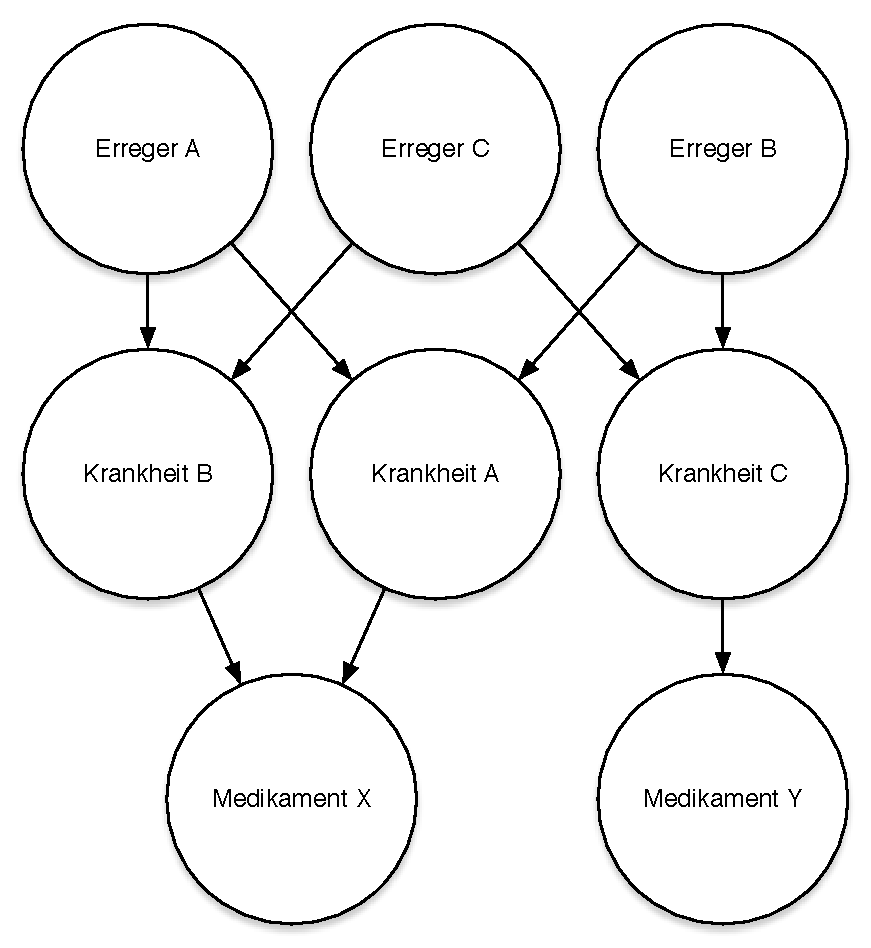
\includegraphics[width=.4\textwidth]{chapters/bayes/bayes_intro.pdf}
    \caption{Beispiel eines Bayesschen Netzes zur Diagnose von Krankheiten (ohne Wahrscheinlichkeiten)}
\end{figure}

\section{Grundlagen der Wahrscheinlichkeitsrechnung}
Einem Ereignis A weisen wir eine Wahrscheinlichkeit p(A) zwischen 0 (tritt nie ein) und 1 (tritt immer ein) zu.

Als marginal probability bezeichnen wir eine Wahrscheinlichkeit p(A), welche keine Abhängigkeiten aufweist.
Beispiel: A = Eine aus einem Skatdeck gezogene Karte ist Kreuz.
p(A) = 1/4 (oder 25~\%)

Als joint probability bezeichnen wir Wahrscheinlichkeiten, welche nebeneinander auftreten. p(A,B)
Beispiel: A (von oben) und B: Die Karte ist ein Bube

Da A und B voneinander unabhängige Ereignisse sind folgt:
p(A,B) = p(A) $\cdot$ p(B) = 1/8 $\cdot$ 1/4 = 1/32

Sind Ereignisse jedoch nicht unabhängig, so müssen wir die Wahrscheinlichkeit von p(A,B) bereits bestimmt haben.
Möchten wir nun für eine große Anzahl Ereignisse Wahrscheinlichkeiten berechnen, so benötigen wir extrem viele Daten.

\begin{center}
\begin{tabular}{ ccccc } \toprule
Sonne scheint & Werktag & Stau & Rasensprinkler & Tage im Jahr \\ \midrule
F & F & F & F & 4 \\
F & F & F & T & 5 \\
F & F & T & F & 2 \\
F & F & T & T & 1 \\
F & T & F & F & 13 \\
F & T & F & T & 2 \\
F & T & T & F & 66 \\
F & T & T & T & ... \\
T & F & F & F & ... \\
T & F & F & T & \\
T & F & T & F & \\
T & F & T & T & \\
T & T & F & F & \\
T & T & F & T & \\
T & T & T & F & \\
T & T & T & T & Errechenbar \\
\bottomrule
\end{tabular}
\end{center}


Bis auf 1 errechenbares Ergebnis benötigen wir die direkten Werte aller Kombinationen.
Wir benötigen also Für N Ereignisse $2^N-1$ Datensätze.
Gerade in der Medizin aus dem Anfangsbeispiel gibt es aber oft extrem viele Ereignisse.

Oftmals ist vieles davon aber auch nicht interessant, bzw. ableitbar.
Die Wahrscheinlichkeit, dass die Sonne scheint ist beispielsweise unabhängig davon ob der Tag ein Werktag ist.

Um die benötigten Datensätze möglichst gering zu halten betrachtet man bedingte Wahrscheinlichkeiten (conditional probability).

\section{Bedingte Wahrscheinlichkeit}
Bedingte Wahrscheinlichkeiten beruhen auf Annahmen.
Man nimmt etwa an, dass die Sonne keinen Einfluss auf die Frage hat, ob es nun ein Werktag ist, sehr wohl jedoch auf die Frage, ob der Sprinkler angeschaltet ist.
Gehen wir weiterhin davon aus, dass an sonnigen Tagen mehr Staus zustande kommen, da z.B. Fahrer geblendet werden.
Zudem gehen wir davon aus, dass werktags mehr Staus auftreten.
Fügen wir zudem noch das Verpassen des Essens hinzu, welches lediglich vom Stau abhängt.

\begin{figure}[h]
    \centering
    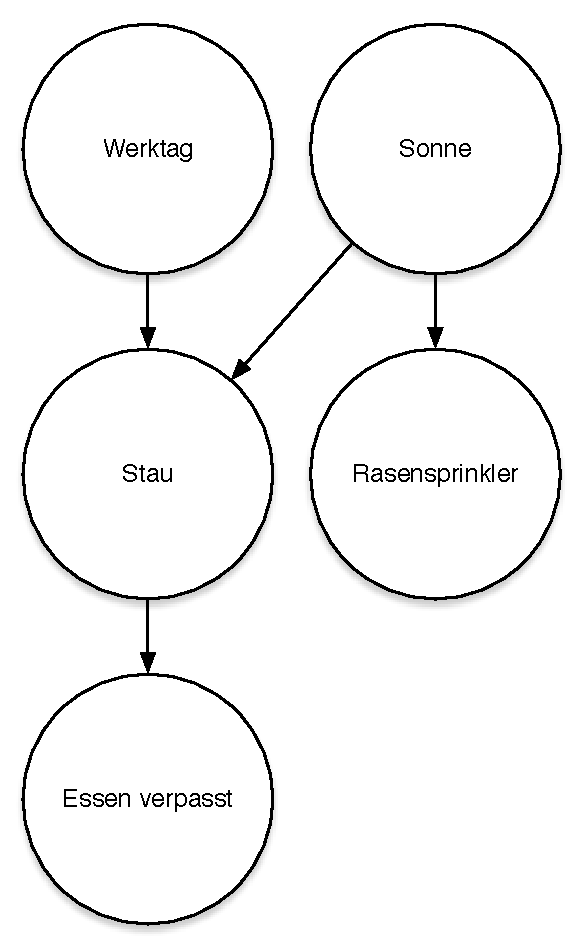
\includegraphics[width=.2\textwidth]{chapters/bayes/bayes_example.pdf}
\end{figure}

Unsere benötigten Datensätze mit fiktivem Inhalt:\\
$p(Sonne) = 0,8$\\
$p(Werktag)= 0,7$\\
$p(Rasensprinkler | Sonne) = 0,95$\\
$p(Rasensprinkler | !Sonne) = 0,20$\\
$p(Stau | Sonne,Werktag) = 0,8$\\
$p(Stau | !Sonne, Werktag) = 0,75$\\
$p(Stau | Sonne, !Werktag) = 0,15$\\
$p(Stau | !Sonne, !Werktag) = 0,05$\\
$p(Essen verpasst | Stau) = 0,5$\\
$p(Essen verpasst | !Stau) = 0,05$\\

Von 31 Datensätzen in einer Tabelle mit joint probabilities haben wir nun nur noch 10 benötigt Wahrscheinlichkeiten und können alle anderen nun problemlos errechnen. (Beispiel folgt)

Um bedingte Wahrscheinlichkeiten effektiv nutzen zu können benötigen wir einige Definitionen:
\begin{equation*}
p(A,B) = p (A | B) \cdot p (B)
\end{equation*}
Daraus folgt direkt:
\begin{equation*}
p(A,B,C) = p(A | B,C) \cdot p(B,C) = p(A | B,C) \cdot p(B | C) \cdot p(C)
\end{equation*}
Dies lässt sich für N Ereignisse wie folgt darstellen (Chain Rule):
\begin{equation*}
    P\left(\bigcap_{k=1}^N A_k\right)  = \prod_{k=1}^N  \mathrm P\left(A_k \,\Bigg|\, \bigcap_{j=1}^{k-1} A_j\right)
\end{equation*}
Zudem bezeichnen wir A als von B unabhängig, wenn gilt:
\begin{equation*}
p(A | B) = p(A)
\end{equation*}
und A als von B unabhängig unter der Prämisse C, wenn gilt:
\begin{equation*}
p(A | C) \cdot p(B | C) = p(A,B | C)
\end{equation*}

Mit Hilfe der Chain-Rule können wir nun für das Beispiel von oben jede mögliche joint probability ausrechnen.

Beispiel:
p(Essen verpasst,Stau,Werktag,Rasensprinkler,Sonne)
nach Anwendung der Chain Rule haben wir:
p(Essen verpasst | Stau,Werktag,Rasensprinkler,Sonne) \\ $\cdot$ p(Stau | Werktag , Rasensprinkler, Sonne) \\ $\cdot$ p(Werktag | Rasensprinkler, Sonne)
\\ $\cdot$ p( Rasensprikler | Sonne)
\\ $\cdot$ p(Sonne)

Wichtig ist hier den Aufbau des ersten Ausdrucks entlang der Abhängigkeiten zu formulieren. Die Reihenfolge der Ereignisse für die joint probabilty muss also eine umgedrehte topologische Anordnung unseres Graphen darstellen bzw. ein Ereignis A kann nicht vor einem Ereignis B stehen, wenn B abhängig von A ist.

Nach dem kürzen der Unabhängigkeiten erhalten wir:
p(Essen verpasst | Stau ) $\cdot$ p( Stau | Werktag, Sonne) $\cdot$ p( Werktag) $\cdot$ p( Rasensprinkler | Sonne) $\cdot$ p(Sonne)

Man nennt dies auch die Faktorisierung.

Die gesuchten Wahrscheinlichkeiten kennen wir bereits und können sie einsetzen:
0,5 $\cdot$ 0,8 $\cdot$ 0,7 $\cdot$ 0,95 $\cdot$ 0,8 = 0,218.

Es ist also durch simples Einsetzen unserer 10 Werte möglich sämtliche 31 Werte für die joint probability Tabelle zu berechnen.
Gleichzeitig sind Lösungen für relevante Fragen zur bedingten Wahrscheinlichkeit, welche nicht alle Ereignisse umfassen, mit geringem Aufwand zu lösen.


In der Regel sind jedoch nicht alle Angaben bekannt.
Nehmen wir nun an, dass wir als hart arbeitender Mensch an einem Nicht-Werktag zur Arbeit fahren und es sonnig ist.
Wir möchten nun wissen, wie wahrscheinlich es ist, dass man es abends bei der Rückfahrt rechtzeitig zum Essen schafft.
Wir suchen also p(!Essen verpasst | !Werktag, Sonne).

Dazu berechnen wir:
p(!Essen verpasst | Stau) $\cdot$ p(Stau | Sonne, Werktag) + p(!Essen verpasst | !Stau) $\cdot$ p(!Stau | Sonne, Werktag)

Die passenden Werte kennen wir entweder oder können sie direkt ableiten.
p(Essen verpasst | Stau) = 0,5
p(Essen verpasst | !Stau) = 0,05
p(Stau | Sonne, !Werktag) = 0,15

0,5 $\cdot$ 0,15 + 0,95 $\cdot$ 0,85 = 0,8825 bzw. die Wahrscheinlichkeit am Wochenende pünktlich zum Essen zu kommen ist 88\%.

Was jedoch, wenn ich in die andere Richtung rechnen möchte?
Beispiel: Der Lebensgefährte kommt pünktlich zum Essen und ich möchte Wissen, wie wahrscheinlich es ist, dass er im Stau gesteckt hat.

Wir kennen bereits die Formel:\\
p(A,B) = p (A | B) $\cdot$ p(B) offensichtlich gilt auch\\
p(B,A) = p (B | A) $\cdot$ p(A) wir folgern daraus:\\
p(A | B) = p(A,B) / P(B) = p(B,A) / P(B) = p(B | A) $\cdot$ p(A)/p(B) (Satz von Bayes)

Wir wissen also:
p(Stau | !Essen verpasst) = p(!Essen verpasst | Stau ) *P(Stau)/p(! Essen verpasst)

p(!Essen verpasst | Stau) =0,5\\
p(Stau) =\\
p(Stau | Sonne, Werktag) $\cdot$ p(Sonne) $\cdot$ p(Werktag) + \\ p(Stau | Sonne, !Werktag) $\cdot$ p(Sonne) $\cdot$ p(!Werktag)+ \\ p(Stau | !Sonne, Werktag) $\cdot$ p(!Sonne) $\cdot$ p(Werktag) + \\ p(Stau | !Sonne, !Werktag) $\cdot$ p(!Sonne) $\cdot$ p(!Werktag)\\ = 0,382

p(!Essen verpasst) =\\
p(!Essen verpasst | Stau) $\cdot$ p(Stau)\\ + p(!Essen verpasst | !Stau) $\cdot$ p(!Stau)\\ = 0,7781

$\Rightarrow$ p(Stau | !Essen verpasst)=0,5 $\cdot$ 0,382/0,7781 = 0,2454...

Ist die Person also pünktlich, so gab es mit einer Wahrscheinlichkeit von ~75\% keinen Stau.

An dieser Stelle ist anzufügen, dass das ganze Problem auch so hätte modelliert werden können, dass die Pünktlichkeit beim Essen ebenfalls vom Werktag abhängig ist, dann jedoch wäre die Abhängigkeit zum Stau zu hinterfragen, wenn es denn keinen Werktag gibt.
Es gibt also durchaus komplexere Problemstellungen, die wir mit unseren einfachen Methoden nicht so einfach behandeln können und eventuell verschiedene Modelle für Abhängigkeiten die je nach der Menge der Daten möglicherweise nicht optimal sind.

Diese neue Methode hilft uns vor allen Dingen damit mit einem einzelnen Modell gleichzeitig z.B. Krankheiten und Symptome in beide Richtungen zu bestimmen. Ohne große Umstände kann eine Krankheit aus Symptomen bestimmt werden und direkt von der Wahrscheinlichkeit der Krankheit kann die Wahrscheinlichkeit für weitere Symptome berechnet werden.

\section{Graphische Darstellung}
\begin{figure}[h]
    \centering
    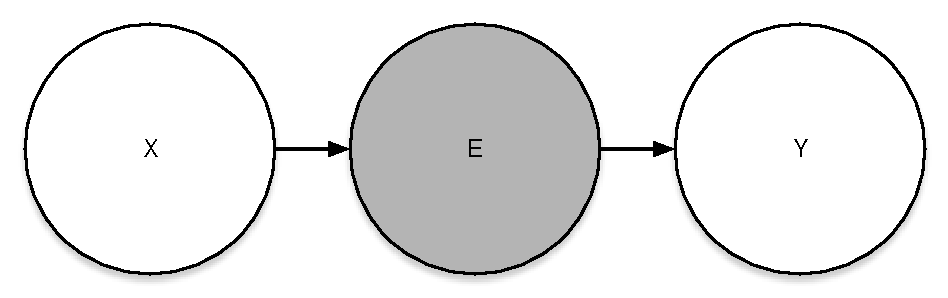
\includegraphics[width=.2\textwidth]{chapters/bayes/bayes_net_1.pdf}
\end{figure}
\begin{figure}[h]
    \centering
    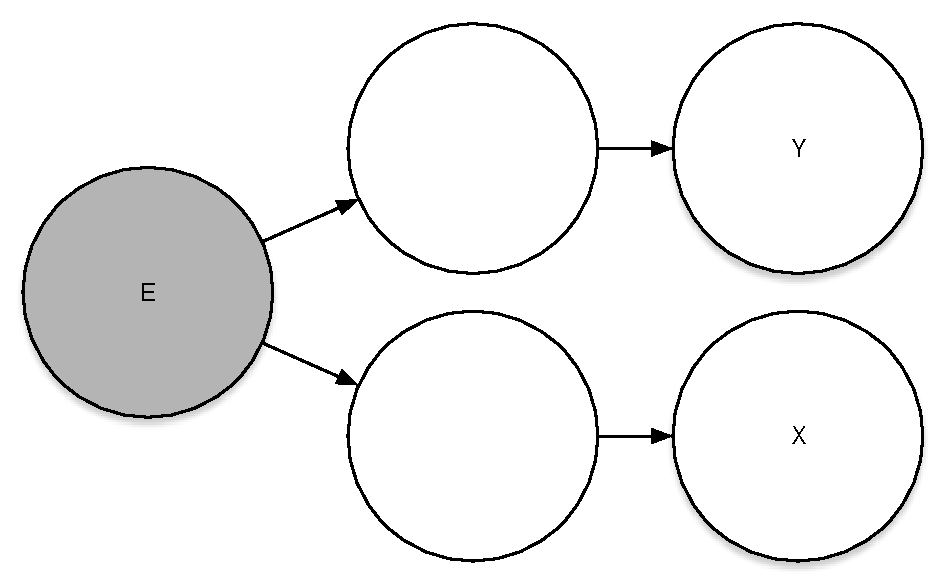
\includegraphics[width=.2\textwidth]{chapters/bayes/bayes_net_2.pdf}
\end{figure}
\begin{figure}[h]
    \centering
    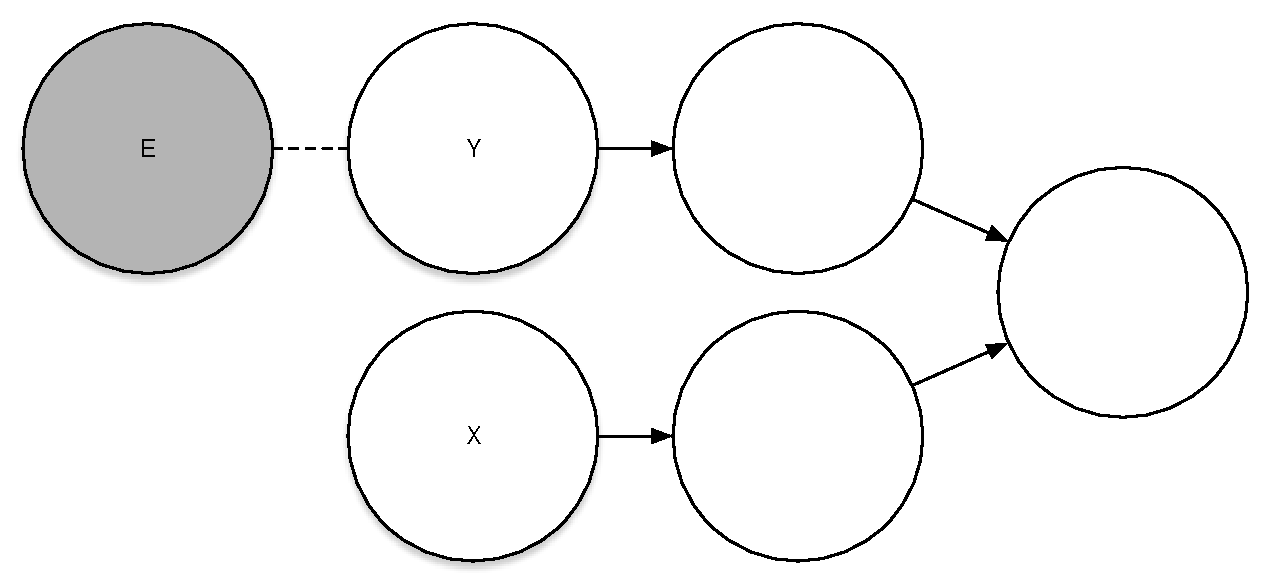
\includegraphics[width=.2\textwidth]{chapters/bayes/bayes_net_3.pdf}
\end{figure}
\begin{figure}[h]
    \centering
    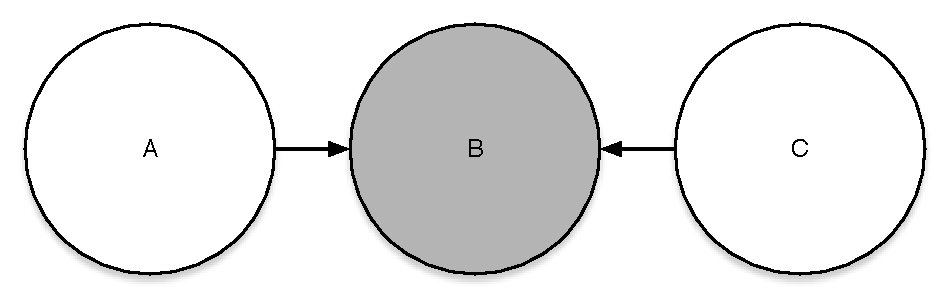
\includegraphics[width=.2\textwidth]{chapters/bayes/bayes_net_4.pdf}
\end{figure}

Wir nennen zwei Ereignisse X und Y bedingt unabhängig gegeben E, wenn im Graphen kein Weg von X zu Y existiert, welcher nicht E nicht beinhaltet.
Dies wir auch d-Separation genannt.
Wir schreiben hierfür
$X \perp Y | E$
Ausgehend vom vorherigen Beispiel heißt das, dass das Verpassen des Essens zwar vom Werktag abhängt, jedoch wenn bekannt ist, ob es einen Stau gab, diese Abhängigkeit aufgehoben wird.
Für 3 verknüpfte Ereignisse gibt es die Folgenden Möglichkeiten:
\begin{enumerate}[label=(\alph*)]
\item $A \rightarrow B \rightarrow C$ impliziert $A \perp C | B$
\item $A \leftarrow B \leftarrow C$ impliziert $A \perp C | B$
\item $A \leftarrow B \rightarrow C$ impliziert $A \perp C | B$
\item $A \rightarrow B \leftarrow C$ impliziert $A \perp C$
\end{enumerate}
Das Beispiel (d) beschreibt hierbei eine sogenannte V-Struktur.

Betrachten wir hierzu außerdem die Verschiedenen Faktorisierungen:
\begin{enumerate}[label=(\alph*)]
\item p(A,B,C) = p(C|B) $\cdot$ p(B|A) $\cdot$ p(A)
\item p(A,B,C) = p(A|B) $\cdot$ p(B|C) $\cdot$ p(C)
\item p(A,B,C) = p(A|B) $\cdot$ p(C|B) $\cdot$ p(B)
\item p(A,B,C) = p(B|A,C) $\cdot$ p(A) $\cdot$ p(C)
\end{enumerate}

\section{IC-Algorithmus}
Der IC Algorithmus ist eine Möglichkeit aus gegebenen Unabhängigkeiten ein Bayessches Netz zu erstellen.
\begin{enumerate}
\item Konstruiere einen ungerichteten Graphen; füge jede mögliche Kante (X,Y), für die es keine (bedingte) Abhängigkeit $X \perp Y | E$ bzw. $X \perp Y$ gibt, in den Graphen ein.
\item Gilt für zwei Nachbarn X,Y von einem Knoten E die bedingte Unabhängigkeit $X \perp Y | E$, dann füge die Kanten (X,E) und (Y,E) hinzu. (V-Struktur)
\item Orientiere die verbleibenden Kanten beliebig, aber ohne neue V-Strukturen entstehen zu lassen.
\end{enumerate}

\section{Quellen}
\begin{itemize}
\item Open Course „Artifical Intelligence“ am MIT
\item https://upload.wikimedia.org/math/b/5/a/b5a87dba9ec79dd6a93628c85fab ca97.png
\item http://www.informatik.uni-bremen.de/tdki/lehre/ss12/bayes/Intro.pdf
\item http://www.fil.ion.ucl.ac.uk/~wpenny/bdb/bayes.pdf
\item Bayesian Artificial Intelligence, Second Edition
\end{itemize}


\part{Suche}
\chapterimage{chapter_head_1.png}

\chapter{Tiefensuche, Beam-Seach und Hill Climbing}

\tikzset{
  treenode/.style = {align=center, inner sep=0pt, text centered,
    font=\sffamily},
  arn_n/.style = {treenode, circle, white, font=\sffamily\bfseries, draw=black,
    fill=black, text width=1.5em},% arbre rouge noir, noeud noir
  arn_r/.style = {treenode, circle, red, draw=red,
    text width=1.5em, very thick},% arbre rouge noir, noeud rouge
  arn_x/.style = {treenode, rectangle, draw=black,
    minimum width=0.5em, minimum height=0.5em}% arbre rouge noir, nil
}

\algnewcommand\algorithmicinput{\textbf{Input:}}
\algnewcommand\INPUT{\item[\algorithmicinput]}

\lstset{language=Haskell,frame=single,basicstyle=\small\ttfamily,numbers=left,firstnumber=1}
\lstset{language=Prolog,frame=single,basicstyle=\small\ttfamily,numbers=left,firstnumber=1}

\section{Motivation}

Die Hauptaufgabe von Rechnern ist, Probleme zu lösen. Oft kann man die Probleme graphisch darstellen, mit einem Start- und einem Zielknoten und die Wege zwichen den beiden. Hierfür benötigt man nicht nur eine Darstellung des aktuellen Zustandes sondern auch die Möglichkeiten, die zur Verfügung stehen, um das Ziel zu erreichen. Meistens gibt es keine einfache Lösung, denn nicht alle Probleme sind Addition von zwei positiven ganzen Zahlen. Daher benötigt man Suchverfahren. Hier beschänken wir uns auf die Depth-First Search, Breadth-First Search, Hill Climbing und Best-First Suchverfahren.

\section{Suchalgorithmen}

Wenn man vom Problem und der Darstellung abstrahiert, kann man die Suche nach einer Lösung in einem gerichteten Graph betrachten. Der gerichtete Graph wird nicht gegeben  sondern wird durch Erzeugungsregeln abgeleitet. Der Graph kann auch unendlich groß sein und daher ist die Suche und partielle Erzeugung des Graphen somit verflochten.

Unser Suchgraph besteht hier aus Knoten, die die Zustände beschreiben, und Kanten, in Form von Funktionen, die die Nachfolgerknoten berechnet. Außerdem definieren wir eine Anfangssituation und ein Ziel.

\begin{tikzpicture}[->,>=stealth',level/.style={sibling distance = 5cm/#1,level distance = 1.5cm}]
\node [arn_n] {S}
    child{ node [arn_n] {}
            child{ node [arn_n] {}
            	child{ node [arn_n] {}}
							child{ node [arn_x] {}}
            }
            child{ node [arn_n] {}
							child{ node [arn_n] {}}
							child{ node [arn_x] {}}
            }
    }
    child{ node [arn_n] {}
            child{ node [arn_n] {}
							child{ node [arn_n] {Z}}
							child{ node [arn_n] {}}
            }
            child{ node [arn_n] {}
							child{ node [arn_n] {}}
							child{ node [arn_x] {}}
            }
    };

    \node [below=5.2cm, align=flush center,text width=8cm]
       {
           Fig1: Graphische Darstellung eines Problems   S: Startknoten, Z: Zielknoten
       };
\end{tikzpicture}

%\subsection{Problemstellung}

%\TODO: Beispiel: Route finding, VLSI Layout, Assembly Sequencing

\section{Uninformierte Suche}
Wir betrachten zunächst die nicht informierte Suche. Hierbei wird bei der Suche nur den Graphen und die Nachfolgerfunktion berücksichtigt, aber keine anderen Informationen über die Knoten, Kanten usw. dürfen verwendet werden.

Die Paramenter für unseren Graph sind

\begin{itemize}
  \item Menge der initialen Knoten
  \item Menge der Zielknoten, bzw eindeutige Festlegung der Eigenschaft der Zielknoten
  \item Nachfolgerfunktion N
\end{itemize}

damit lässt sich folgender Algorithmus schreiben:

\begin{algorithm}
\caption{General-Search Algorithm}
\begin{algorithmic}[1]
\Function{General-Search}{problem,strategy} \State \textbf{returns} a solution, or failure
\State initialize the search tree using the initial state of $problem$
\Loop \State choose a leaf node for expansion according to $strategy$
  \If {there are no candidates for expansion}{failure}
  \If{the node contains a goal state}{the corresponding solution}
  \Else{expand the node and add the resulting nodes to the search tree}
\EndLoop
\EndFunction
\end{algorithmic}
\end{algorithm}


Wir betrachten im folgenden Varianten der blinden Suche, die insbesondere das Wählen des Knotens eindeutig durchführen.

\subsection{Depth-First Search}
Die Depth-First Suche verwendet eine Liste von Knoten und wählt als nächsten zu betrachtenden Knoten dieser Liste. Außerdem werden neue Nachfolger vorne in die Liste eingefügt, was zur Charakteristik führt, dass zunächst in der Tiefe gesucht wird.

\begin{algorithm}
\caption{Depth-First Search Algorithm}
\begin{algorithmic}[1]
\Function{Depth-First-Search}{problem} \State \textbf{returns} a solution, or failure
\Function{General-Search}{problem,Enqueue-At-Front}
\EndFunction
\EndFunction
\end{algorithmic}
\end{algorithm}

Die Depth-First Suche eignet sich damit besonders für Suchbäume, deren Äste eine vertretbare Länge nicht überschreiten.

\begin{tikzpicture}[->,>=stealth',level 1/.style={sibling distance=50mm},level 2/.style={sibling distance=20mm},level 3/.style={sibling distance=12mm},
%scale=1.2, transform shape
]
\node (nA)[arn_n] {A}
   child { node (nB)[arn_n] {B}
              child { node (nD) [arn_n] {D}
                         child { node (nH) [arn_n] {H} }
                       }
              child {  node (nE) [arn_n] {E}
                         child { node (nI) [arn_n] {I} }
                         child { node (nJ) [arn_n] {J} }
                       }
            }
   child { node (nC) [arn_n] {C}
              child { node (nF) [arn_n] {F}
                         child { node (nK) [arn_n] {K}  }
                         child { node (nL) [arn_n] {L} }
                         child { node (nM) [arn_n] {M} }
                       }
              child {  node (nG) [arn_n] {G} }
             };

  \draw[->,blue,rounded corners,dashed,line width=0.7pt]
    ($(nA) + (-0.4,0.2)$) --
    ($(nB) +(-0.3,0.4)$) --
    ($(nB) +(-0.6,0.0)$) --
    ($(nD)  +(-0.4,0.3)$) --
    ($(nD)  +(-0.5,0.0)$) --
    ($(nH)  +(-0.5,0.0)$) --
    ($(nH)  +(-0.4,-0.35)$) --
    ($(nH)  +(0.0,-0.5)$) --
    ($(nH)  +(0.4,-0.35)$) --
    ($(nH)  +(0.5,0.0)$) --
%    ($(nD)  +(0.45,-0.2)$) --
    ($(nD)  +(0.45,0.0)$) --
    ($(nB)  +(0.0,-0.4)$) --
    ($(nE)  +(-0.45,0.0)$) --
    ($(nI)  +(-0.45,0.0)$) --
    ($(nI)  +(-0.35,-0.35)$) --
    ($(nI)  +(0.0,-0.45)$) --
    ($(nI)  +(0.35,-0.35)$) --
    ($(nI)  +(0.4,0.0)$) --
    ($(nE)  +(0.0,-0.4)$) --
    ($(nJ)  +(-0.45,0.0)$) --
    ($(nJ)  +(-0.35,-0.35)$) --
    ($(nJ)  +(0.0,-0.45)$) --
    ($(nJ)  +(0.35,-0.35)$) --
    ($(nJ)  +(0.45,0.0)$) --
    ($(nE)  +(0.4,0.2)$) --
    ($(nB)  +(0.4,0.0)$) --
    ($(nA)  +(0.0,-0.4)$) --
    ($(nC)  +(-0.4,0.0)$) --
%    ($(nF)  +(-0.6,0.0)$) --
    ($(nK)  +(-0.5,0.1)$) --
    ($(nK)  +(-0.4,-0.35)$) --
    ($(nK)  +(0.0,-0.5)$) --
    ($(nK)  +(0.4,-0.3)$) --
    ($(nF)  +(-0.15,-0.4)$) --
    ($(nL)  +(-0.5,0.0)$) --
    ($(nL)  +(-0.4,-0.35)$) --
    ($(nL)  +(0.0,-0.5)$) --
    ($(nL)  +(0.4,-0.35)$) --
    ($(nL)  +(0.5,0.0)$) --
    ($(nF)  +(0.15,-0.4)$) --
    ($(nM)  +(-0.5,0.0)$) --
    ($(nM)  +(-0.4,-0.35)$) --
    ($(nM)  +(0.0,-0.5)$) --
    ($(nM)  +(0.4,-0.35)$) --
    ($(nM)  +(0.5,0.2)$) --
    ($(nF)  +(0.4,0.0)$) --
    ($(nC)  +(0.0,-0.4)$) --
    ($(nG)  +(-0.5,0.0)$) --
    ($(nG)  +(-0.4,-0.35)$) --
    ($(nG)  +(0.0,-0.5)$) --
    ($(nG)  +(0.4,-0.35)$) --
    ($(nG)  +(0.5,0.1)$) --
    ($(nC) +(0.6,0.0)$) --
    ($(nC) +(0.3,0.4)$) --
    ($(nA) + (0.4,0.2)$);

    \node [below=5.4cm, align=flush center,text width=8cm]
       {
           Fig2: Graphische Darstellung der Depth-First Suche
       };
\end{tikzpicture}

Eine mögliche Implementierung der Depth-First Suche in Prolog ist:


\lstinputlisting[language=Prolog]{chapters/dfs/tiefensuche.pl}

Und in Haskell:

\lstinputlisting[language=Haskell]{chapters/dfs/tiefensuche.hs}

Die explizite Speicherung der Pfade sowohl in Haskell als auch in Prolog kostet nicht viel Effizienz. Man kann den Algorithmus auch in imperativen Sprachen implementieren, indem jeder Eintrag einen Knoten mit Zeiger auf den nächsten Nachbarknoten zugeordnet wird. Die Komplexität des Verfahrens (worst-case) für die Zeit ist entsprechend der Anzahl der besuchten Knoten exponentiell in der Tiefe und für den Speicherplatz linear bei fester Verzweigungsrate.

Das Problem bei der Depth-First Suche ist, dass der Algorithmus nicht vollständig ist. Wenn der Suchgraph unendlich groß ist, kann die Suche am Ziel vorbeilaufen und für immer im unendlichen langen Pfad laufen.

Um dies zu verbeugen kann man eine Tiefenbeschränkung (k) einbauen. Wenn die vorgegebene Tiefenschrank (k) überschriten wird, werden keine Nachfolger dieser Knoten mehr erzeugt. Die Depth-First Suche findet in diesem Fall jeden Zielknoten, der höchstens Tiefe k hat.

Wenn der gerichtete Graph kein Baum ist, kann man auch die schon untersuchten Knoten in einer Hash-Tabelle speichern und somit werden die Knoten nicht nochmal untersucht sondern redundant weiterverfolgt.

Hierfür ist der Platzbedarf entsprechend der Anzahl der besuchten Knoten und die Berechnungszeit gleich $n*log(n)$ mit n = Anzahl der untersuchten Knoten.

\subsubsection{Backtracking}
Die Arbeitsweise der Depth-First Suche ist: Wenn Knoten K keine Nachfolger hat (oder eine Tiefenbeschränkung) überschritten wurde, dann mache weiter mit dem nächsten Bruder von K. Ist der Pfad nicht erfolgreich, führt die Depth-First Suche Backtracking durch. Dies wird als chronologisches Zurücksetzen bezeichnet.

Es gibt auch Suchprobleme, bei denen kein Backtracking erforderlich ist (greedy Verfahren ist möglich) zum Beispiel, wenn jeder Knoten noch einen Zielknoten als Nachfolger hat. Die Depth-First Suche reicht dann aus, wenn die Tiefe der Zielknoten in alle Richtungen unterhalb jedes Knotens beschränkt ist. Anderenfalls reicht Depth-First Suche nicht aus, da ein Ast immer ausgesucht werden kann, indem der Zielknoten weiter weg ist.

\subsection{Breadth-First Search}
Die Breadth-First Suche verwendet auch eine Liste von Knoten wie bei der Depth-First Suche. Der Unterschied hierbei ist, dass die neuen Nachfolger hinten in die Liste eingefügt werden, was zur Charakteristik führt, dass zunächst in der Breite gesucht wird.

\begin{algorithm}
\caption{Breadth-First Search Algorithm}
\begin{algorithmic}[1]
\Function{Breadth-First-Search}{problem} \State \textbf{returns} a solution, or failure
\Function{General-Search}{problem,Enqueue-At-End}
\EndFunction
\EndFunction
\end{algorithmic}
\end{algorithm}

Die Breadth-First Suche untersucht somit ausgehend von Startknoten alle Nachbarknoten. Ist der Zielknoten noch nicht erreicht, werden alle Nachbarknoten der bisher untersuchten Knoten betrachtet.

\begin{tikzpicture}[->,>=stealth',level 1/.style={sibling distance=50mm},level 2/.style={sibling distance=20mm},level 3/.style={sibling distance=12mm},
%scale=1, transform shape
]
\node (nA)[arn_n] {A}
   child { node (nB)[arn_n] {B}
              child { node (nD) [arn_n] {D}
                         child { node (nH) [arn_n] {H} }
                       }
              child {  node (nE) [arn_n] {E}
                         child { node (nI) [arn_n] {I} }
                         child { node (nJ) [arn_n] {J} }
                       }
            }
   child { node (nC) [arn_n] {C}
              child { node (nF) [arn_n] {F}
                         child { node (nK) [arn_n] {K}  }
                         child { node (nL) [arn_n] {L} }
                         child { node (nM) [arn_n] {M} }
                       }
              child {  node (nG) [arn_n] {G} }
             };

  \draw[->,blue,rounded corners,dashed,line width=0.7pt]
    ($(nA) + (-0.4,0.2)$) --
    ($(nB) +(-0.3,0.4)$) --
    ($(nB) +(-0.6,0.0)$) --
    ($(nC)  +(+0.3,0.2)$) --
    ($(nC)  +(+0.6,0.0)$) --
    ($(nD)  +(-0.3,0.4)$) --
    ($(nD)  +(-0.4,0.0)$) --
    ($(nE)  +(0.0,0.0)$) --
    ($(nE)  +(0.0,0.0)$) --
    ($(nF)  +(0.0,0.0)$) --
    ($(nF)  +(0.0,0.0)$) --
    ($(nG)  +(0.3,0.2)$) --
    ($(nG)  +(+0.6,0.0)$) --
    ($(nH)  +(-0.3,0.4)$) --
    ($(nH)  +(0.0,0.0)$) --
    ($(nI)  +(0.0,0.0)$) --
    ($(nI)  +(0.0,0.0)$) --
    ($(nJ)  +(0.0,0.0)$) --
    ($(nJ)  +(0.0,0.0)$) --
    ($(nK)  +(0.0,0.0)$) --
    ($(nK)  +(0.0,0.0)$) --
    ($(nL)  +(0.0,0.0)$) --
    ($(nL)  +(0.0,0.0)$) --
    ($(nM)  +(+0.5,0.0)$);

    \node [below=5.2cm, align=flush center,text width=8cm]
       {
           Fig3: Graphische Darstellung der Breadth-First Suche
       };
\end{tikzpicture}

Eine mögliche Implementierung der Breadth-First Suche in Prolog ist:

\lstinputlisting[language=Prolog]{chapters/dfs/breitensuche.pl}

Und in Haskell:

\lstinputlisting[language=Haskell]{chapters/dfs/breitensuche.hs}

Die Vor- und Nachteile der Breadth-First Suche lässt sich wie folgt zusammenfassen:

\begin{itemize}
  \item Die Breadth-First Suche ist vollständig. Das bedeutet, wenn es eine Lösung gibt, wird sie mit Sicherheit gefunden.
  \item Der kürzeste Weg wird gefunden, dafür wird aber viel Speicherplatz benötigt.
  \item Es werden Knoten besucht, die für den optimalen Pfad nicht besucht werden müssten. Damit wird auch der Zeitaufwand erhöht. Dies beträgt nämlich $n+n*log(n)$, für n = Anzahl der Knoten.
\end{itemize}

\subsection{Reverse Search}
Bei der Rückwärtssuche wird von einem (bekannten) Zielknoten ausgegangen in die Richtung des Anfangsknoten.

Voraussetzungen für die Rückwärtssuche sind:

\begin{itemize}
  \item Der Zielknoten kann explizit angeben werden(nicht nur eine Eigenschaft, die der Zielknoten erfüllen muss).
  \item Von jedem Knoten ist es möglich, die direkten Vorgänger zu berechnen.
\end{itemize}

Reverse Suche ist aber nur besser als Vorwärtssuche, wenn die Verzweigungsrate in Rückwärtsrichtung kleiner ist als die Verzweigungsrate in Vorwärtsrichtung. Das Problem an der Reverse Suche ist oft, dass die Vorgängerfunktion schwer zu finden ist.

\section{Informierte Suche}

Die Algorithmen, die bis jetzt betrachtet wurden, erzeugen neuen Zuständen und vergleichen sie immer wieder mit dem Zielzustand, bis sie übereinstimmen. Diese Strategie funktioniert, ist aber oft sehr kostenaufwendig. Wir betrachten im folgenden heuristischen Algorithmen.

Die Suche wird als \enquote{heuristische} oder \enquote{informierte} bezeichnet, wenn man zusätzlich zu den Knoten und zu der Datenstruktur eine Schätzfunktion gibt, die als Schätzung des Abstands zum Zielknoten interpretieren werden kann. Der Zielknoten sollte ein Maximum bzw. Minimum der Schätzfunktion sein.

Eine Heuristik ist dann eine Methode, die oft ihren Zweck erreicht, aber nicht mit Sicherheit. Man spricht von heuristischer Suche, wenn die Schätzfunktion in vielen praktisch brauchbaren Fällen die richtige Richtung zu einem Ziel angibt, aber möglicherweise manchmal versagt.

Wir suchen dann das Maximum (oder Mininum) einer Knotenfunktion auf einem gerichteten Graphen.

\subsection{Hill Climbing}
Der Hill Climbing Suchalgorithm ist auch als Gradientenaufstieg bekannt, da die Suche immer in Richtung der Vergrößerung einer Funktion läuft.

Parameter, die notwendig für den Algorithmus sind:

\begin{itemize}
  \item die Menge der initialen Knoten,
  \item die Nachfolgerfunktion,
  \item die Schätzfunktion,
  \item und der Zieltest.
\end{itemize}

Der Algorithmus verhält sich wie die Depth-First Suche, wobei der Nachfolger, der zu expandieren ist, nach der Schätzfunktion ausgesucht wird.

\begin{algorithm}
\caption{Hill Climbing Algorithm}
\begin{algorithmic}[1]
\Function{Hill-Climbing}{problem} \State \textbf{returns} a solution state
\INPUT
\Statex $problem$ \Comment Ein Problem
\Statex $current$  \Comment Ein Knoten
\Statex $next$  \Comment Ein Knoten
\State $current \gets Make-Node(Initial-State[problem])$
\Loop
\State $next \gets$ größter Wert aus $current$
\If{$VALUE[next] < VALUE[current]$}{\Return current}
\State $current \gets next$
\EndLoop
\EndFunction
\end{algorithmic}
\end{algorithm}


Das Problem bei dem Hill Climbing Algorithmus ist, dass er bei lokalen Maxima abbricht. Es ist möglich, in dem Hill-Clinbing Algorithmus Zyklen einzubauen, damit Backtracking durchgeführt wird, aber er bleibt eine zeitlang in den Maxima hängen.

Wenn mehrere Nachfolger die gleiche Schätzwerte haben, ist der Weg, den ausgesucht werden soll, nicht eindeutig.

Eine mögliche Implementierung der Hill Climbing Suche in Haskell ist:

\lstinputlisting[language=Haskell]{chapters/dfs/hillclimbing.hs}

\subsection{Best-First-Search}
Die Best-First-Suche wählt immer den Knoten aus, der den besten Wert bzgl. der Schätzfunktion hat. Der Knoten wird dann überprüft und, wenn der nicht das Ziel ist, expandiert.


\begin{algorithm}
\caption{Best-First-Search Algorithm}
\begin{algorithmic}[1]
\Function{Best-First-Search}{problem,EVAL-FN} \State \textbf{returns} a solution sequence
\INPUT
\Statex $problem$ \Comment Ein Problem
\Statex $Eval-Fn$  \Comment Eine Evaluationsfunktion
\State $Queueing-Fn \gets$ a function that orders nodes by EVAL-FN
\State \textbf{return} GENERAL-SEARCH(problem, Queueing-Fn)
\EndFunction
\end{algorithmic}
\end{algorithm}


Eine Implementierung der Best-First Suche in Haskell ist:

\lstinputlisting[language=Haskell]{chapters/dfs/bestfirst.hs}

Die Best-First-Suche ist mit der Depth-First Suche eng verbunden. Der Unterschied ist, dass bei der Best-First Suche den nächsten Knoten, der überprüft und expandiert wird, mithilfe der Schätzfunktion ausgesucht wird. Dabei werden alle Knoten im Stack bewertet und dadurch können lokale Maxima schnell verlassen werden.

Wie bei der Depth-First Suche ist die Best-First Suche hier nicht vollständig und die Platzkosten steigern exponentiell in der Tiefe.

\section{Fazit \& Bewertung}
Zunächst wurden das Suchproblem und der Begriff \enquote{Suche} erläutert. Die nicht informierte Suchverfahren wurden präsentiert und es wurde gezeigt, dass ein General Search Algorithmus alle Probleme löst, wenn die richtige Strategie ausgesucht wird.
Tiefensuche bedeutet, dass man beginnend im Startknoten so weit wie möglich entlang der bestehenden Kanten in die Tiefe geht, ehe man zurückläuft und dann in bislang unbesuchte Teilbäume absteigt.
Breitensuche bedeutet, dass man beginnend im Startknoten alle direkt verbundenen Knoten besucht, bevor die nächst tiefere Ebene überprüft wird.
Die Vollständigkeit und die Komplexität der gängigen uninformierten Suchalgorithmen wurden erläutert.
Dabei ist klar geworden, dass die Zeit- und Speicherplatzkosten hoch sind.

Um die Kosten zu minimieren werden die bekannte Suchverfahren weiterentwickelt. Daraus folgte zum Beispiel die Best-First Suche. Diese ist eine General Search, wobei nur die minimale Anzahl der Knoten berücksichtigt wird.

Solche Algorithmen, wobei die Kosten minimiert werden, nennen wir \textbf{greedy Algorithmen}. Der Algorithmus ist aber immer noch nicht optimal.

\section{Quellen und Literatur}

\begin{itemize}
\item Stuart J. Russel and Peter Norvig, “Artificial Intelligence - A Modern Approach”, Pretince Hall, Englewood Cliffs, New Jersey 2010
\item Ivan Bratko, “Prolog Programming for Artificial Intelligence”, Addison-Wesley Yugoslavia 1990
\item R. Schenk and R.P. Abelson, “Scripts, Plans and Knowledge”, International Joint Conference on Artificial Intelligence, 1975
\item F.C. Pereira and S.M.Schieber, “Prolog and Natural-Language Analysis”, CSLI, 1987
\item F.M. Donini, M. Lenzerini and others, “The complexity of concept languages”, Inf. Comput., 1997
\item I. Wegener, “Highlights aus der Informatik”, Springer, Berlin, 1996
\item MIT Open Course - Artificial Intelligence
 \url{http://ocw.mit.edu/courses/electrical-engineering-and-computer-science/6-034-artificial-intelligence-fall-2010/}, Zugriff 28.04.2016
\end{itemize}

\chapterimage{chapter_head_1.png}

\chapter{Suchalgorithmen für Spiele}

\usetikzlibrary{calc}
\usetikzlibrary{positioning}
\usetikzlibrary{matrix}

\pgfdeclarelayer{background}
\pgfsetlayers{background,main}


\section{Intro \& Motivation}

In den vorangegangenen Kapiteln haben wir schon einige Suchverfahren kennengelernt, welche uns nun helfen werden Algorithmen zu verstehen, die verwendet werden um Computergegner für Nullsummenspiele zu entwickeln. Hierbei werden wir uns den Minimax-Algorithmus, sowie den Alpha-Beta-Algorithmus genauer anschauen, welche beide versuchen sich in die Lage des Gegners zu versetzen, um so  herauszufinden, welche Reaktion dieser auf einen Zug von uns wählen würde. Ziel der Algorithmen ist es, ein für uns best mögliches Ergebnis und somit, wenn möglich, einen Sieg zu erlangen. Dieses Vorgehen kann eine Betrachtung von sehr vielen möglichen Züge zur Folge haben, was sehr viel Rechenaufwand bedeutet. Im Folgenden werden wir jedoch  mit Hilfe des Alpha-Beta-Algorithmus eine Methode kennenlernen, die es uns ermöglicht die Anzahl der zu betrachtenden Züge zu reduzieren.



\section{Inhaltliche Ausarbeitung des Themas}

Wir betrachten ein Nullsummenspiel, was bedeutet, dass der Gewinn des einen Spielers (Nutzwert positiv) mit dem Verlust des Gegners (Nutzwert negativ) äquivalent ist und ein Unentschieden keine Auswirkungen auf die Nullsummeneigenschaft hat (Nutzwert 0).
Gegeben sei für dieses Spiel ein Spielbaum $T = (V;E)$. Bei einem gleichförmigen Spielbaum besitzt jeder innerer Knoten den gleichen Verzweigungsgrad b und alle Blätter befinden sich in der gleichen Tiefe d, , sodass die Zahl der Knoten in einem gleichförmigen Baum exponentiell mit der Tiefe des Baumes wächst ($b^d$). Jedoch gibt es auch Spielbäume bei denen der Verzweigungsgrad der Ebenen variiert.
Der Spielbaum beinhaltet alle möglichen Züge und Spielausgänge. Die Tiefe und der Verzweigungsgrad hängt von dem Spiel ab, welches wir betrachten. Beispielsweise hat der Spielbaum zu einem Tic-Tac-Toe Spiel eine Tiefe von 9 (da es 9 Felder zu besetzen gibt) und zu Beginn des Spiels einen Verzweigungsgrad von 9 (weil noch alle 9 Felder zur Auswahl stehen), der mit wachsender Tiefe allerdings abnimmt, da nach jedem Zug immer ein leeres Feld weniger vorhanden ist.



\subsection{Problemstellung}
Zu dem gegeben Nullsummenspiel wollen wir einen Computergegner programmieren, der in der Lage ist die optimale Antwort auf jede Spielposition, bei optimalem Spiel beider Spieler, zu finden.
Dafür müssen wir jedoch vorher festlegen, was für uns optimal in diesem Zusammenhang bedeutet. Wir gehen davon aus, dass der Gegner immer den für ihn optimalen Zug wählt, dh der Zug, der für ihn zum besten Nutzwert und somit für uns zum schlechtesten Nutzwert führt. Analog wollen wir agieren. Wie dies genau funktioniert werden wir im folgenden Abschnitt sehen.



\subsection{Methoden}


\subsubsection*{Minimax Algorithmus}
Im folgenden bezeichnen wir unseren Spieler mit MAX und den gegnerischen Spieler mit MIN. Wie zuvor schon angedeutet ist das Ziel des Minimax Algorithmus den Minimax-Wert für die aktuelle Stellung zu bestimmen. Der Minimax-Wert der Endstellungen (Blätter) entspricht dem Nutzwert für MAX. Die Berechnung der anderen Knoten erfolgt rekursiv mit Hilfe der folgenden Bewertungsfunktion:

\begin{center}
	$Minimax(k) = \begin{cases} Nutzwert(k) &		,falls~ k ~Endzustand\\
		max\{minimax(t) ~|~ t \in N(t)\} 	&		,falls~ k~ MAX-Knoten\\
		min\{minimax(t) ~|~ t \in N(t)\},	&		,falls~ k~ MIN-Knoten	\end{cases} $
\end{center}

wobei $N(t)$ die Funktion ist, die die Kinder im Baum liefert. Die Auswertung der Knoten geschieht Bottom up, das bedeutet wir beginnen bei den Blättern und bewerten von dort ausgehend die Elternknoten und anschließend deren Eltern bis wir irgendwann bei der Wurzel angelangt sind. Der Minimax Algorithmus liefert nicht unbedingt den höchsten Nutzwert der Blätter, sondern den größten Nutzwert den man erhalten kann, wenn der Gegner selbst versucht zu gewinnen und somit den Nutzwert für uns möglichst klein zu halten.\\

Anschaulicher wird das ganze, wenn man sich den Algorithmus an einem Beispiel anschaut.

\textbf{Beispiel}\\

Gegeben sei der folgende Spielbaum
\begin{center}
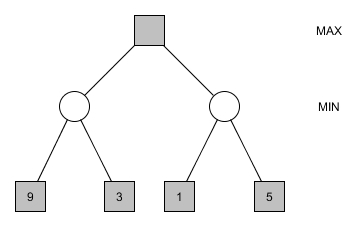
\includegraphics[width = 7 cm]{chapters/minimax/jpg/Graph-Minmax1.jpg}
\end{center}

Angenommen MIN wäre an der markierten Position:
\begin{center}
	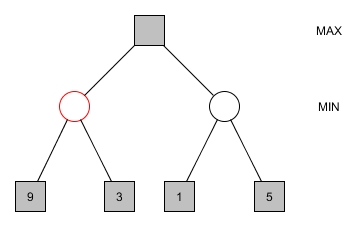
\includegraphics[width = 7 cm]{chapters/minimax/jpg/Graph-Minmax2-1.jpg}
\end{center}

Dann würde MIN den Zug auswählen, der für ihn den größten Nutzwert und somit für uns den kleinsten Nutzwert hat. Das heißt in dem Fall:
\begin{center}
	 $min\{minimax(t) | t \in N(t)\} ~=~ min\{9,3\} ~=~ 3$

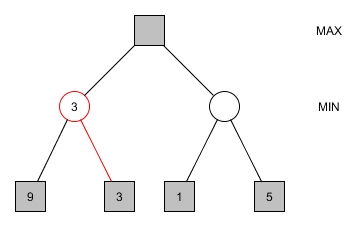
\includegraphics[width = 7 cm]{chapters/minimax/jpg/Graph-Minmax2-2.jpg}
\end{center}

Angenommen MIN wäre an der markierten Position:
\begin{center}
	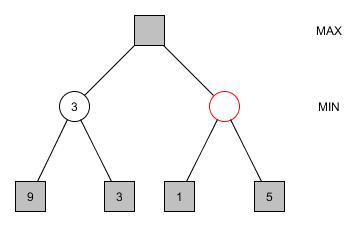
\includegraphics[width = 7 cm]{chapters/minimax/jpg/Graph-Minmax2-3.jpg}
\end{center}

Dann würde MIN den Zug auswählen, der für ihn den größten Nutzwert und somit für uns den kleinsten Nutzwert hat. Das heißt in dem Fall:
\begin{center}
	$min\{minimax(t) | t \in N(t)\} ~=~ min\{1,5\} ~=~ 1$

	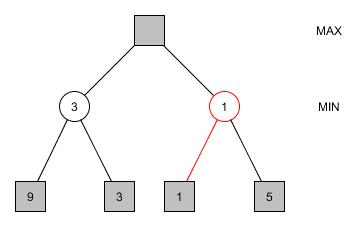
\includegraphics[width = 7 cm]{chapters/minimax/jpg/Graph-Minmax2-4.jpg}
\end{center}

Nun betrachten wir den Zug von MAX. Der Suchbaum sieht wie folgt aus

\begin{center}
	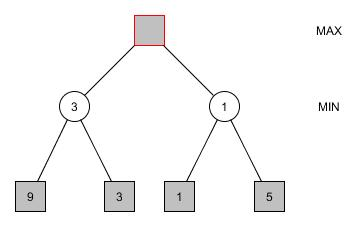
\includegraphics[width = 7 cm]{chapters/minimax/jpg/Graph-Minmax2.jpg}
\end{center}

MAX würde den Zug wählen, der für ihn den höchsten Nutzwert hat.\\

\begin{center}
	$max\{minimax(t) | t \in N(t)\} ~=~ max\{3,1\} ~=~ 3$
	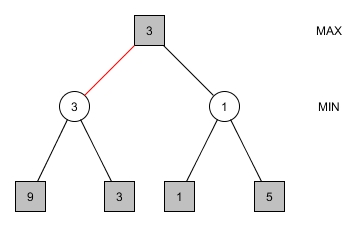
\includegraphics[width = 7 cm]{chapters/minimax/jpg/Graph-Minmax3.jpg}
\end{center}

Somit sieht der Suchbaum nach Abschluss des Minimax-Algorithmus wie folgt aus, wobei der rote Pfad den optimalsten Nutzwert liefert, wenn beide Spieler optimal spielen. Somit sollte MAX den linken Knoten wählen.

\begin{center}
	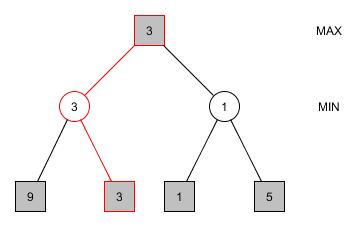
\includegraphics[width = 7 cm]{chapters/minimax/jpg/Graph-Minmax4.jpg}
\end{center}

\vskip 60pt



\subsubsection*{Problem:} Der Minimax-Algorithmus durchsucht den Suchbaum $T=(V, E)$ mit Tiefensuche, in der Zeit $O(max {|V|, |E|}) = O(|V|)$. Somit benötigt die Suche zwar lineare Zeit, jedoch wächst der Baum exponentiell mit zunehmender Tiefe ($O(|V|)=O(b^d)$). Somit ist der Algorithmus für Bäume mit großer Tiefe ineffizient.


\subsubsection*{Alpha-Beta-Algorithmus}
 Der Alpha-Beta-Algorithmus ist eine Verbesserung vom Minimax-Algorithmus, da die Zugriffsanzahl reduziert wird, indem Teile des Suchbaums nicht durchsucht werden, ohne dabei das Ergebnis zu verfälschen. Für die Umsetzung werden die Variablen $\alpha$ und $\beta$ eingeführt, wobei $\alpha$ der Nutzwert ist, welchen MAX mindestens erreicht und $\beta$ der Nutzwert, den MIN höchstens erreicht. Die Auswertung der Knoten geschieht on-the-fly, dh nur dann wenn wir sie wirklich benötigen. \\

 \underline{MAX-Knoten:}\\
 Betrachten wir einen MAX Knoten und stellen dort einen Wert fest der größer ist als $\beta$ brauchen wir den Teilbaum nicht weiter betrachten, da MIN diesen nicht wählen würde, weil der andere Teilbaum einen kleineren Nutzwert liefert. Das nicht weiter Betrachten des Teilbaums bezeichnet man als Beta-Cutoff. Ist  der Wert des MAX Knoten größer als $\alpha$ erhöht sich der Wert den MAX mindestens erreicht und wir aktualisieren $\alpha$ auf den Wert des Knotens.  \\

 \underline{MIN-Knoten:}\\
 Ist der Wert eines MIN Knotens kleiner als der Wert von $\alpha$ müssen wir diesen Teilbaum nicht weiter analysieren, da MAX immer den Teilbaum mit dem größten Nutzwert auswählt und da $\alpha$ größer ist als der Wert des betrachteten Knotens existiert ein Teilbaum mit einem größeren Nutzwert. Also würde hier ein Cutoff stattfinden, welchen man als Alpha-Cutoff bezeichnet. Sollte jedoch der Wert des MIN Knotens größer als $\beta$ sein steigt der Wert den MIN höchstens erreicht und wir müssen $\beta$ auf diesen Wert anpassen.


 \begin{algorithm}
 	\KwData{Graph $G=(V,E)$, Blätter mit Nutzwert, s = Knoten}
 	\KwResult{Nutzwert für jeden knoten}
 	\textbf{alpha-beta-suche(s)}\\

 	\textbf{return} maximalerWert(s, -$\infty$, $\infty$)\\

 	\textbf{maximalerWert}(Knoten, $\alpha$, $\beta$)\\

	 	\If{s = Blatt}{
	 		\textbf{return} wert(s)
	 	}
	 	\Else{
	 		$wert = \alpha$\\
	 		\lForEach{k= Kind(s)}{
		 		$wert = max\{wert, minimalerWert(k, wert, \beta)\}$\\
		 		\If {$wert >= \beta$}{
			 		\textbf{return} wert}
			 	$\alpha = max\{\alpha, wert\}$\\
	 		\textbf{return} wert
	 		}
	 	}

	\textbf{minimalerWert}(Knoten, $\alpha$, $\beta$)\\

	\If{s = Blatt}{
		\textbf{return} wert(s)
	}
	\Else{
		$wert = \beta$\\
		\lForEach{k= Kind(Knoten)}{
			$wert = min\{wert, minimalerWert(k, \alpha, wert)\}$\\
			\If {$wert <= \alpha$}{
				\textbf{return} wert}
			$\beta = min\{\beta, wert\}$\\
			\textbf{return} wert
		}
	}
 	\caption{Alhpa-Beta-Algorithmus}
\end{algorithm}

Betrachten wir ein Beispiel, um den Algorithmus besser zu verstehen.

\textbf{Beispiel:}\\

Gegeben sei der folgende Spielbaum:
\begin{center}
	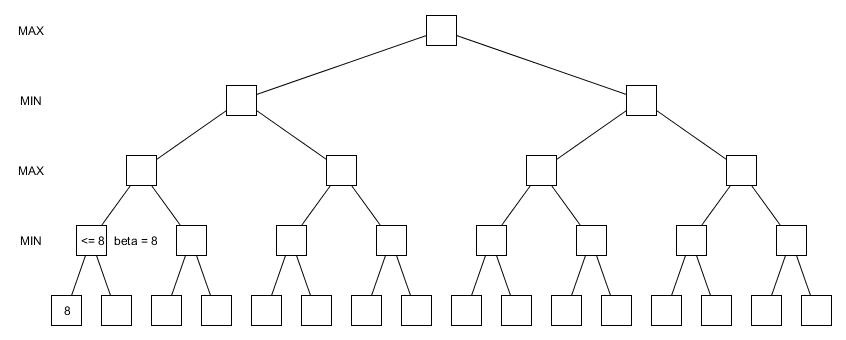
\includegraphics[width = 12 cm]{chapters/minimax/jpg/Alpha-beta1.jpg}
\end{center}

Wir betrachten das erste Blatt. Da MIN immer den Zug mit dem niedrigsten Nutzwert auswählt erreicht er einen Nutzwert $<=8$. Somit ist $\beta = 8$. Da $\beta > \alpha = -\infty$ müssen wir noch das andere Blatt betrachten.

\begin{center}
	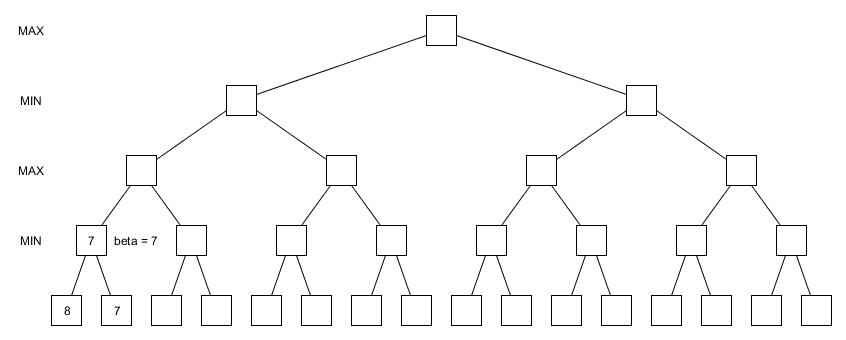
\includegraphics[width = 12 cm]{chapters/minimax/jpg/Alpha-beta2.jpg}
\end{center}

Das zweite Blatt hat den Nutzwert 7, somit ist er kleiner als der aktuelle Wert von $\beta$. Aus diesem Grund erhält der MIN-Knoten den Wert $min\{8,~7\} =7$. Somit ergibt sich für den darüberliegenden Knoten, dass er einen Wert $>=7$ hat, da MAX immer den Knoten mit dem größten Nutzwert auswählt. Nun betrachten wir das Blatt mit dem Nutzwert 3.

\begin{center}
	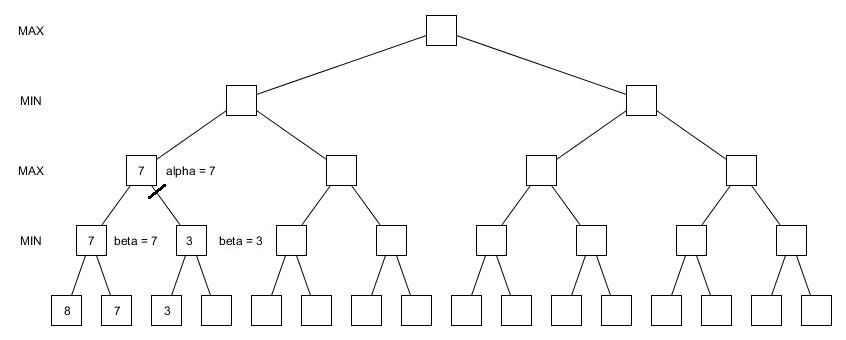
\includegraphics[width = 12 cm]{chapters/minimax/jpg/Alpha-beta3.jpg}
\end{center}

Sein Elternknoten hat für $\alpha$ den Wert 7 (MAX erreicht mind. eine 7) und $\beta$ hat den Wert 3 (MIN erreicht höchstens den Wert 3). Vergleicht man $\alpha$ und den Wert des MIN Knotens fällt auf, dass $\alpha$ > 3 was bedeutet, dass man den Teilraum nicht weiter betrachten muss und hier ein Cutoff durchgeführt wird. Anders ausgedrückt MAX würde nicht diesen Zug wähle, da der andere Zug einen Nutzwert von 7 liefert und dieser nur einen von maximal 3.

\begin{center}
	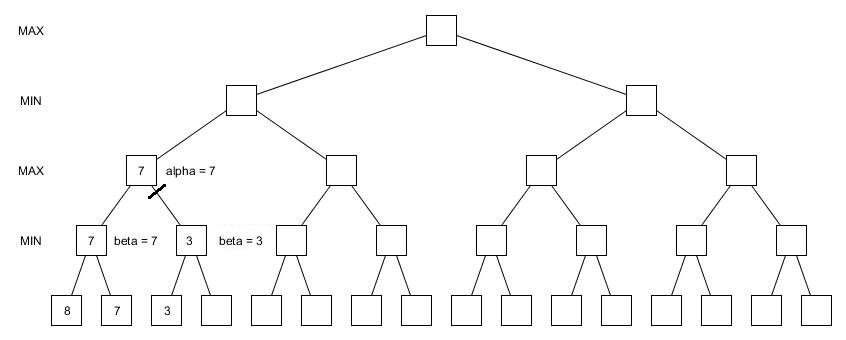
\includegraphics[width = 12 cm]{chapters/minimax/jpg/Alpha-beta3-1.jpg}
\end{center}

Somit erreicht MAX an dem Knoten einen Nutzwert von 7 und der darüber liegende MIN Knoten einen Wert von $<=7$, was bedeutet, dass $\beta = 7$. Betrachten wir nun das nächste Blatt, welches den Nutzwert 9 hat.

\begin{center}
	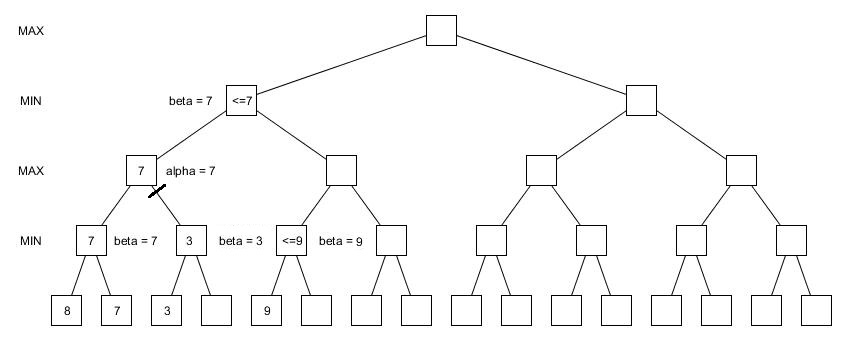
\includegraphics[width = 12 cm]{chapters/minimax/jpg/Alpha-beta4.jpg}
\end{center}

 Da $-\infty = \alpha <9$ müssen wir auch das nächste Blatt betrachten. Anders ausgedrückt, wir können nicht ausschließen das MIN das rechte Blatt wählen würde.

 \begin{center}
 	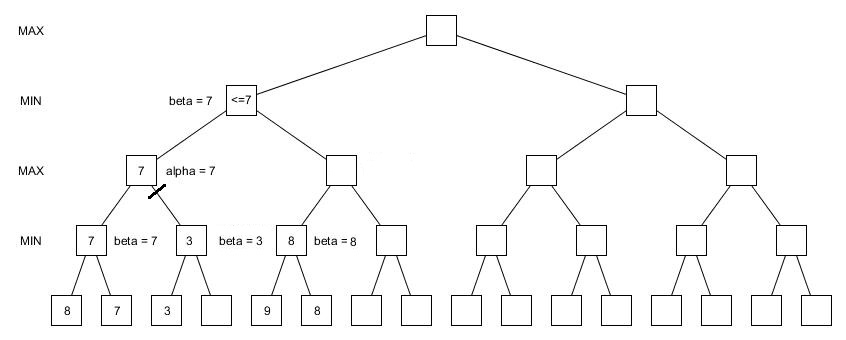
\includegraphics[width = 12 cm]{chapters/minimax/jpg/Alpha-beta5.jpg}
 \end{center}

 Da das nächste Blatt den Nutzwert 8 hat, würde MIN diesen Zug wählen, da sein Nutzwert kleiner ist als der des anderen Zuges ($min\{\beta, 8\}= min\{9,8\}=8$). Somit aktualisiert sich der Wert von $\beta$ auf 8.

 \begin{center}
 	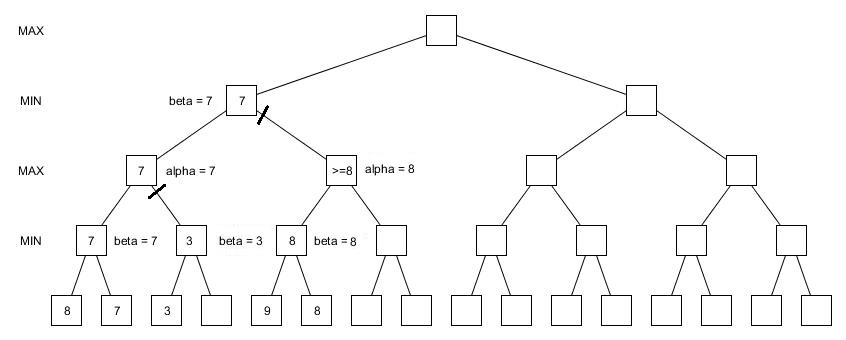
\includegraphics[width = 12 cm]{chapters/minimax/jpg/Alpha-beta6.jpg}
 \end{center}

 Dies hat zur Folge das $\alpha =8$, da MAX im darüber liegenden Zug mindestens einen Nutzwert von 8 erreicht. Somit hat er einen größeren Wert als der linke MAX Knoten, weshalb sich MIN nicht den rechten Knoten aussuchen würde und wir somit auch den Teilbaum nicht weiter betrachten müssen. Anders ausgedrückt, da für den rechten Teilbaum der MAX Knoten einen Wert von mindestens 8 hat und  $\beta = 7$ ist, gilt $\beta<8$ und es findet ein Cutoff statt.  Aufgrund dessen hat der MIN Knoten den Wert 7.

 \begin{center}
 	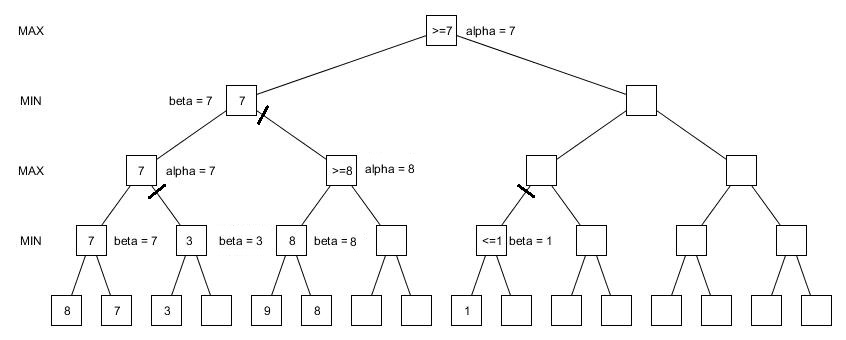
\includegraphics[width = 12 cm]{chapters/minimax/jpg/Alpha-beta7.jpg}
 \end{center}

 Für die Wurzel ergibt sich somit ein Wert von mindestens 7 und $\alpha = 7$
 Die Betrachtung des nächsten Blattes liefert das der MIN Knoten höchstes den Wert 1 hat. Da 1 <$\alpha$ ist eine weitere Betrachtung des Teilbaumes nicht nötig und wir können ihn abschneiden. Mit anderen Worten würde MAX nicht den Zug dieses Teilbaumes wählen, da der Nutzwert des linken Teilbaumes einen höheren Nutzwert hat.

 \begin{center}
 	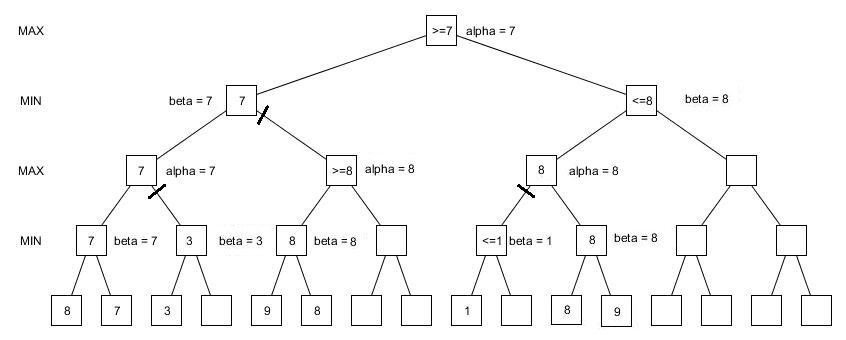
\includegraphics[width = 12 cm]{chapters/minimax/jpg/Alpha-beta8.jpg}
 \end{center}

 Die Auswertung der nächsten beiden Blätter und ihres Elternknotens liefert keine Cutoffs.

 \begin{center}
 	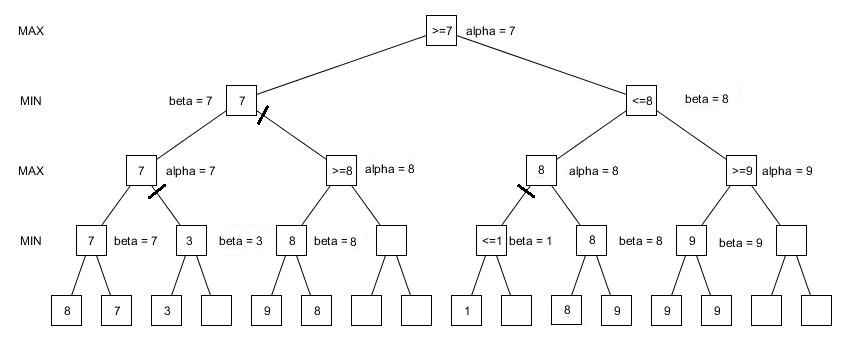
\includegraphics[width = 12 cm]{chapters/minimax/jpg/Alpha-beta9.jpg}
 \end{center}

 Betrachtet man nun die nächsten beiden Blätter liefert das einen Nutzwert von 9 für den MIN Knoten ($\beta =9$) und somit für den MAX Knoten einen Wert $>=9$. Der darüber liegende MIN Knoten würde jedoch nicht den rechten Knoten mit einem Nutzwert $>=9$ wählen, da der linke Knoten nur einen Nutzwert von 8 hat. Somit ist eine weitere Betrachtung des Teilbaumes nicht nötig.\\
 Dies ist somit der endgültige Spielbaum.

 \begin{center}
 	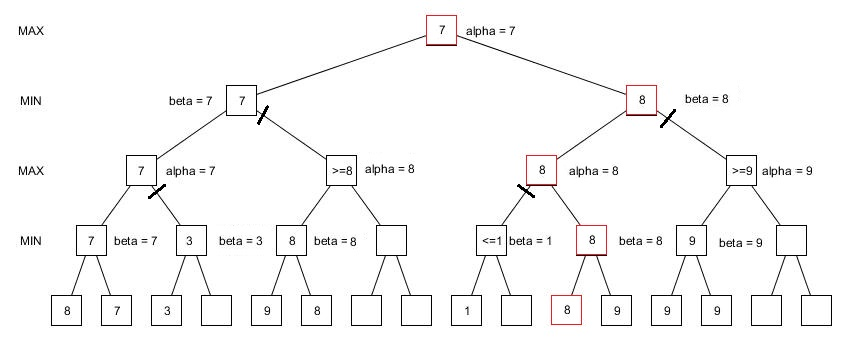
\includegraphics[width = 12 cm]{chapters/minimax/jpg/Alpha-beta10.jpg}
 \end{center}

 Der rot gekennzeichnete Pfad ist der Pfad, der den höchsten Nutzwert liefert, wenn beide Spieler, so wie von uns zu Beginn angenommen, optimal Spielen. Dies bedeutet für den ersten Zug von MAX, dass er den rechten Knoten wählen sollte.

 Für die Berechnung dieses Pfades mussten wir uns 23 Knoten anschauen, wohingegen wir beim Minimax-Algorithmus alle 31 Knoten hätten betrachten müssen, um zu diesem Ergebnis zu gelangen. Somit bietet der Alpha-Beta-Algorithmus in diesem Beispiel eine deutliche Rechenzeitverbesserung.

\section{Abgrenzung / Vergleich zu den vorherigen Kapitel}

In den vorherigen Kapiteln haben wir verschiedene Suchalgorithmen (Bestensuche, Branch-and-Bound, A*) kennengelernt. Diese liefern den Pfad, der zu dem Blatt mit dem höchsten Nutzwert führt. Jedoch beachten sie nicht, ob der Gegner auch diesen Pfad wählen würde. Der Gegner würde versuchen den geringsten Nutzwert für uns zu erreichen und somit versuchen von diesem Pfad abzuweichen.Folglich würden sie keine realistische Einschätzung darüber geben, welche Züge das beste Spielergebnis liefern. Im Gegensatz dazu betrachten sowohl der Minimax, als auch der Alpha-Beta Algorithmus das Verhalten des Gegners, welches zu einer guten Einschätzung der Spielsituation führt.



\section{Fazit \& Bewertung}

Zusammenfassend lässt sich sagen, dass der Minimax- und der Alpha-Beta-Algorithmus zum selben besten Ergebnis für den MAX Spieler führen und sich lediglich in ihrer Effizienz unterscheiden können, da der Alpha-Beta-Algorithmus weniger Berechnungen und somit eine kürzere Rechnungszeit benötigen kann. Je nach Suchbaum kann die Anzahl der Cutoffs und die Einsparung der Rechenzeit sehr groß ausfallen. Aufgrund dessen ist der Alpa-Beta-Algorithmus eine Grundlage für viele Algorithmen im Bereich der Nullsummenspiele für zwei Personen. Für die Berechnungen der Algorithmen sind die Werte der Blätter von größer Bedeutung, welche durch die Heuristik gegeben sind. Alles in allem kann man sagen, dass man sowohl mit Minimax als auch mit Alpha Beta einen Computergegner programmieren kann, der es einem Menschen sehr schwer, wenn nicht sogar unmöglich, macht zu gewinnen und somit eine künstliche Intelligenz bei Nullsummenspielen für die Zukunft denkbar ist.


\section{Quellen und Literatur}

\begin{itemize}
\item MIT - Lecture 6: Search: Games, Minimax, and Alpha-Beta
\item http://home.in.tum.de/~adorf/pub/alphabeta-seminar-paper.pdf
\item https://de.wikipedia.org/wiki/Minimax-Algorithmus
\item https://de.wikipedia.org/wiki/Alpha-Beta-Suche
\end{itemize}


\part{Constraints}

\part{Lernende Systeme}

\part{Sprachverarbeitung}

\part{Philosophische Grundlagen}

%%------------------------------------------------
%
%\section{Citation}\index{Citation}
%
%This statement requires citation \cite{book_key}; this one is more specific \cite[122]{article_key}.
%
%%------------------------------------------------
%
%\section{Lists}\index{Lists}
%
%Lists are useful to present information in a concise and/or ordered way\footnote{Footnote example...}.
%
%\subsection{Numbered List}\index{Lists!Numbered List}
%
%\begin{enumerate}
%\item The first item
%\item The second item
%\item The third item
%\end{enumerate}
%
%\subsection{Bullet Points}\index{Lists!Bullet Points}
%
%\begin{itemize}
%\item The first item
%\item The second item
%\item The third item
%\end{itemize}
%
%\subsection{Descriptions and Definitions}\index{Lists!Descriptions and Definitions}
%
%\begin{description}
%\item[Name] Description
%\item[Word] Definition
%\item[Comment] Elaboration
%\end{description}
%
%%----------------------------------------------------------------------------------------
%%	CHAPTER 2
%%----------------------------------------------------------------------------------------
%
%\chapter{In-text Elements}
%
%\section{Theorems}\index{Theorems}
%
%This is an example of theorems.
%
%\subsection{Several equations}\index{Theorems!Several Equations}
%This is a theorem consisting of several equations.
%
%\begin{theorem}[Name of the theorem]
%In $E=\mathbb{R}^n$ all norms are equivalent. It has the properties:
%\begin{align}
%& \big| ||\mathbf{x}|| - ||\mathbf{y}|| \big|\leq || \mathbf{x}- \mathbf{y}||\\
%&  ||\sum_{i=1}^n\mathbf{x}_i||\leq \sum_{i=1}^n||\mathbf{x}_i||\quad\text{where $n$ is a finite integer}
%\end{align}
%\end{theorem}
%
%\subsection{Single Line}\index{Theorems!Single Line}
%This is a theorem consisting of just one line.
%
%\begin{theorem}
%A set $\mathcal{D}(G)$ in dense in $L^2(G)$, $|\cdot|_0$.
%\end{theorem}
%
%%------------------------------------------------
%
%\section{Definitions}\index{Definitions}
%
%This is an example of a definition. A definition could be mathematical or it could define a concept.
%
%\begin{definition}[Definition name]
%Given a vector space $E$, a norm on $E$ is an application, denoted $||\cdot||$, $E$ in $\mathbb{R}^+=[0,+\infty[$ such that:
%\begin{align}
%& ||\mathbf{x}||=0\ \Rightarrow\ \mathbf{x}=\mathbf{0}\\
%& ||\lambda \mathbf{x}||=|\lambda|\cdot ||\mathbf{x}||\\
%& ||\mathbf{x}+\mathbf{y}||\leq ||\mathbf{x}||+||\mathbf{y}||
%\end{align}
%\end{definition}
%
%%------------------------------------------------
%
%\section{Notations}\index{Notations}
%
%\begin{notation}
%Given an open subset $G$ of $\mathbb{R}^n$, the set of functions $\varphi$ are:
%\begin{enumerate}
%\item Bounded support $G$;
%\item Infinitely differentiable;
%\end{enumerate}
%a vector space is denoted by $\mathcal{D}(G)$.
%\end{notation}
%
%%------------------------------------------------
%
%\section{Remarks}\index{Remarks}
%
%This is an example of a remark.
%
%\begin{remark}
%The concepts presented here are now in conventional employment in mathematics. Vector spaces are taken over the field $\mathbb{K}=\mathbb{R}$, %however, established properties are easily extended to $\mathbb{K}=\mathbb{C}$.
%\end{remark}
%
%%------------------------------------------------
%
%\section{Corollaries}\index{Corollaries}
%
%This is an example of a corollary.
%
%\begin{corollary}[Corollary name]
%The concepts presented here are now in conventional employment in mathematics. Vector spaces are taken over the field $\mathbb{K}=\mathbb{R}$, %however, established properties are easily extended to $\mathbb{K}=\mathbb{C}$.
%\end{corollary}
%
%%------------------------------------------------
%
%\section{Propositions}\index{Propositions}
%
%This is an example of propositions.
%
%\subsection{Several equations}\index{Propositions!Several Equations}
%
%\begin{proposition}[Proposition name]
%It has the properties:
%\begin{align}
%& \big| ||\mathbf{x}|| - ||\mathbf{y}|| \big|\leq || \mathbf{x}- \mathbf{y}||\\
%&  ||\sum_{i=1}^n\mathbf{x}_i||\leq \sum_{i=1}^n||\mathbf{x}_i||\quad\text{where $n$ is a finite integer}
%\end{align}
%\end{proposition}
%
%\subsection{Single Line}\index{Propositions!Single Line}
%
%\begin{proposition}
%Let $f,g\in L^2(G)$; if $\forall \varphi\in\mathcal{D}(G)$, $(f,\varphi)_0=(g,\varphi)_0$ then $f = g$.
%\end{proposition}
%
%%------------------------------------------------
%
%\section{Examples}\index{Examples}
%
%This is an example of examples.
%
%\subsection{Equation and Text}\index{Examples!Equation and Text}
%
%\begin{example}
%Let $G=\{x\in\mathbb{R}^2:|x|<3\}$ and denoted by: $x^0=(1,1)$; consider the function:
%\begin{equation}
%f(x)=\left\{\begin{aligned} & \mathrm{e}^{|x|} & & \text{si $|x-x^0|\leq 1/2$}\\
%& 0 & & \text{si $|x-x^0|> 1/2$}\end{aligned}\right.
%\end{equation}
%The function $f$ has bounded support, we can take $A=\{x\in\mathbb{R}^2:|x-x^0|\leq 1/2+\epsilon\}$ for all $\epsilon\in\intoo{0}{5/2-\sqrt{2}}$.
%\end{example}
%
%\subsection{Paragraph of Text}\index{Examples!Paragraph of Text}
%
%\begin{example}[Example name]
%\lipsum[2]
%\end{example}
%
%%------------------------------------------------
%
%\section{Exercises}\index{Exercises}
%
%This is an example of an exercise.
%
%\begin{exercise}
%This is a good place to ask a question to test learning progress or further cement ideas into students' minds.
%\end{exercise}
%
%%------------------------------------------------
%
%\section{Problems}\index{Problems}
%
%\begin{problem}
%What is the average airspeed velocity of an unladen swallow?
%\end{problem}
%
%%------------------------------------------------
%
%\section{Vocabulary}\index{Vocabulary}
%
%Define a word to improve a students' vocabulary.
%
%\begin{vocabulary}[Word]
%Definition of word.
%\end{vocabulary}
%
%%----------------------------------------------------------------------------------------
%%	PART
%%----------------------------------------------------------------------------------------
%
%\part{Part Two}
%
%%----------------------------------------------------------------------------------------
%%	CHAPTER 3
%%----------------------------------------------------------------------------------------
%
%\chapterimage{chapter_head_1.png} % Chapter heading image
%
%\chapter{Presenting Information}
%
%\section{Table}\index{Table}
%
%\begin{table}[h]
%\centering
%\begin{tabular}{l l l}
%\toprule
%\textbf{Treatments} & \textbf{Response 1} & \textbf{Response 2}\\
%\midrule
%Treatment 1 & 0.0003262 & 0.562 \\
%Treatment 2 & 0.0015681 & 0.910 \\
%Treatment 3 & 0.0009271 & 0.296 \\
%\bottomrule
%\end{tabular}
%\caption{Table caption}
%\end{table}
%
%%------------------------------------------------
%
%\section{Figure}\index{Figure}
%
%\begin{figure}[h]
%\centering
\includegraphics[scale=0.5]{placeholder}
%\caption{Figure caption}
%\end{figure}
%
%%----------------------------------------------------------------------------------------
%%	BIBLIOGRAPHY
%%----------------------------------------------------------------------------------------

\chapter*{Bibliography}
\addcontentsline{toc}{chapter}{\textcolor{hhublue}{Bibliography}}
\section*{Bücher}
\addcontentsline{toc}{section}{Books}
\printbibliography[heading=bibempty,type=book]
\section*{Artikel}
\addcontentsline{toc}{section}{Articles}
\printbibliography[heading=bibempty,type=article]

%----------------------------------------------------------------------------------------
%	INDEX
%----------------------------------------------------------------------------------------

\cleardoublepage
\phantomsection
\setlength{\columnsep}{0.75cm}
\addcontentsline{toc}{chapter}{\textcolor{hhublue}{Index}}
\printindex

%----------------------------------------------------------------------------------------

\end{document}
